\documentclass[10pt]{beamer}
\setbeamertemplate{navigation symbols}{}%remove navigation symbols
\usepackage{booktabs}
\usepackage[FIGTOPCAP]{subfigure}
\usepackage{caption}
\usepackage{lmodern}
\usepackage[T1]{fontenc}
\useoutertheme{infolines}
\usepackage[framemethod=tikz]{mdframed}
\usetikzlibrary{shadows}
\newmdenv[shadow=true,shadowcolor=black,font=\sffamily,rightmargin=8pt]{shadedbox}
\usepackage{pifont,xcolor}% http://ctan.org/pkg/{pifont,xcolor}
\definecolor{myblue}{RGB}{0,29,119}
\usepackage{amsthm}
\usepackage{framed}
\colorlet{shadecolor}{gray!10}
  
\newcommand{\lenitem}[2][.55\linewidth]{\parbox[t]{#1}{#2\strut \strut}}
\usetheme{Frankfurt}

   \usefonttheme{professionalfonts} 
\setbeamertemplate{itemize items}[circle]

\newenvironment{variableblock}[3]{%
  \setbeamercolor{block body}{#2}
  \setbeamercolor{block title}{#3}
  \begin{block}{#1}}{\end{block}}
\usecolortheme{dove}
\usepackage{fancybox}
\setbeamercolor{block title}{bg=white,fg=black}
\newenvironment{fminipage}%
{\begin{Sbox}\begin{minipage}}%
{\end{minipage}\end{Sbox}\fbox{\TheSbox}}

\newcommand{\itemcolor}[1]{% Update list item colour
  \renewcommand{\makelabel}[1]{\color{#1}\hfil ##1}}

\newcounter{tmpc}
%\usefonttheme{structuresmallcapsserif}
\setbeamercolor{section in head/foot}{fg=black, bg=white}

\setbeamertemplate{frametitle}
{
    \nointerlineskip
    \begin{beamercolorbox}[sep=0.3cm,ht=1.8em,wd=\paperwidth]{frametitle}
        \vbox{}\vskip-3ex%
        \strut\insertframetitle\strut
        \vskip-1.2ex%
    \end{beamercolorbox}
}
\addtobeamertemplate{frametitle}{\vskip0.5ex}{}
\makeatletter
\setbeamertemplate{footline}
{
  \leavevmode%
  \hbox{%
  \begin{beamercolorbox}[wd=.875 \paperwidth,ht=2.25ex,dp=1ex,left]{section in head/foot}%
    \usebeamerfont{author in head/foot}\quad \quad \insertshorttitle
 \end{beamercolorbox}%
 \begin{beamercolorbox}[wd=.125\paperwidth,ht=2.25ex,dp=1ex,right]{section in head/foot}%
    \usebeamerfont{date in head/foot}\insertshortdate \quad \quad
    \insertframenumber{} / \inserttotalframenumber\hspace*{2ex} 
  \end{beamercolorbox}}%
  \vskip0pt%
}
\makeatother

\section{Introduction}
\subsection{Subsection}


\begin{document}

\title{A Guide to Using EViews for your MSc Dissertation}
\date{}
\author{Charles Rahal}%l\\ \small{Research Fellow\\ University of Birmingham/University of Oxford}}
\frame{\titlepage 
\begin{center}
\vspace{-0.75in}
Slides Available: \color{blue}\url{http://github.com/crahal}\color{black}\\ \vspace{0.1in}
%For comments or suggestions: \url{r.c.rahal@bham.ac.uk}\\ \vspace{0.1in}
%Please note: all work here is \color{red}\textbf{extremely preliminary}\color{black}.\\ \vspace{0.35in}
\small
%\texttt{A few slides given at the TSRC-NCVO-CSDP event in Manchester \\ 
\vspace{0.1in}
\texttt{Last Updated: 21st June, 2016}
\end{center}
}



\frame{\frametitle{Outline of this Session}
By the end of this session, you should be able to...:\\[0.1in] 
\begin{enumerate}
\item[1.] Section One: Introduction.\\[0.05in]
\item[2.] Section Two: Import and plot data from a .xls or .csv file.\\[0.05in]
\item[3.] Section Three: Using databases and transforming data.\\[0.05in]
\item[4.] Section Four: Use and understand the invaluable `add-ins' feature.\\[0.05in]
\item[5.] Section Five: Run Simple OLS Regression.\\[0.05in]
\item[6.] Section Six: Undertake a basic forecasting exercise.\\[0.05in]
\item[7.] Section Seven: VAR and VECM models. \\[0.05in]
%\item[8.] Section Eight: Volatility Models. \\[0.05in]
\item[8.] Section Eight: Write some programs for repetative tasks.\\[0.05in]
\item[9.] Section Nine: Optional Homework Assignment.\\[0.5in]
\end{enumerate}
}

\frame{\frametitle{More Advanced Delegates}
\begin{center}
\begin{shaded}If you're already an advanced EViews user/econometrician and require a further challenge - please feel free to skip to the `Optional Homework Question' at the end of the slides.\end{shaded}
\end{center}
}


\frame{\frametitle{Textbooks and supplementary material}
\begin{itemize} 
\item No textbook adequately covers all the material here.\\[0.1in]
\item These slides are sufficient to help you get started with the software, although you'll have to modify and expand the methods to your specific topic.\\[0.1in]
\item One of the main strengths of EViews is the forum support:\\[0.1in]
\begin{center}
\color{blue}\url{forums.eviews.com}\color{black}
\end{center}
\item Registration is free and EViews staff (as well as members of public including top academics) will often help anybody seeking assistance.\\[0.1in]
\item Please try not to ask people to do your work for you. If you're going to ask a general econometric theory question -- be sure to use the correct subform. In general, try to only ask about Eviews functionality, and provide information on what you have already tried.\\[0.1in]
\item Say hello to `CharlieEVIEWS' if you see him there!
\end{itemize}
}


\frame{\frametitle{Textbooks and supplementary material (Cont.)}
\begin{itemize} 
\item The excellent user guides/accompanying documentation ship with most versions of EViews and are also available in licensed computer labs:
\begin{figure}
    \scalebox{.15}{
\includegraphics{eviewsuserguidescreen.png}}
\end{figure}
\item There is a \textbf{FREE} textbook endorsed by EViews:
\begin{center}
\color{blue}\url{www.eviews.com/illustrated/EViews_Illustrated.pdf}\color{black}
\end{center}
written by Professor Richard Startz (``startz'' on EViews forums) at UC Santa Barbara. \textbf{This textbook is \textcolor{red}{very comprehensive}!}
\end{itemize}
}



\frame{\frametitle{Introduction to EViews}
\begin{itemize}
\item EViews is one of the most widely used econometrics softwares, especially within universities and central banks.\\[0.2in]
\item Very accessible `front-end' menu driven interface, which is heavily object-orientated (e.g. groups, graphs, tables, matrices, vectors are all objects.)\\[0.2in]
\item This is combined with a powerful command line, program and batch mode, allowing customization and replication.\\[0.2in]
\item Written in C++, owned by IHS (global information/analytics company), but no knowledge of CS or programming required.\\[0.2in]
\item Especially powerful for time-series, economic modeling, financial econometrics and forecasting.\\[0.2in]
\end{itemize}
}


\frame{\frametitle{Introduction to EViews (Cont)}
\begin{itemize} 
\item The interface works like this, and is fairly self explanatory:\\
\end{itemize}
\begin{center}
\begin{figure}
    \scalebox{.2}{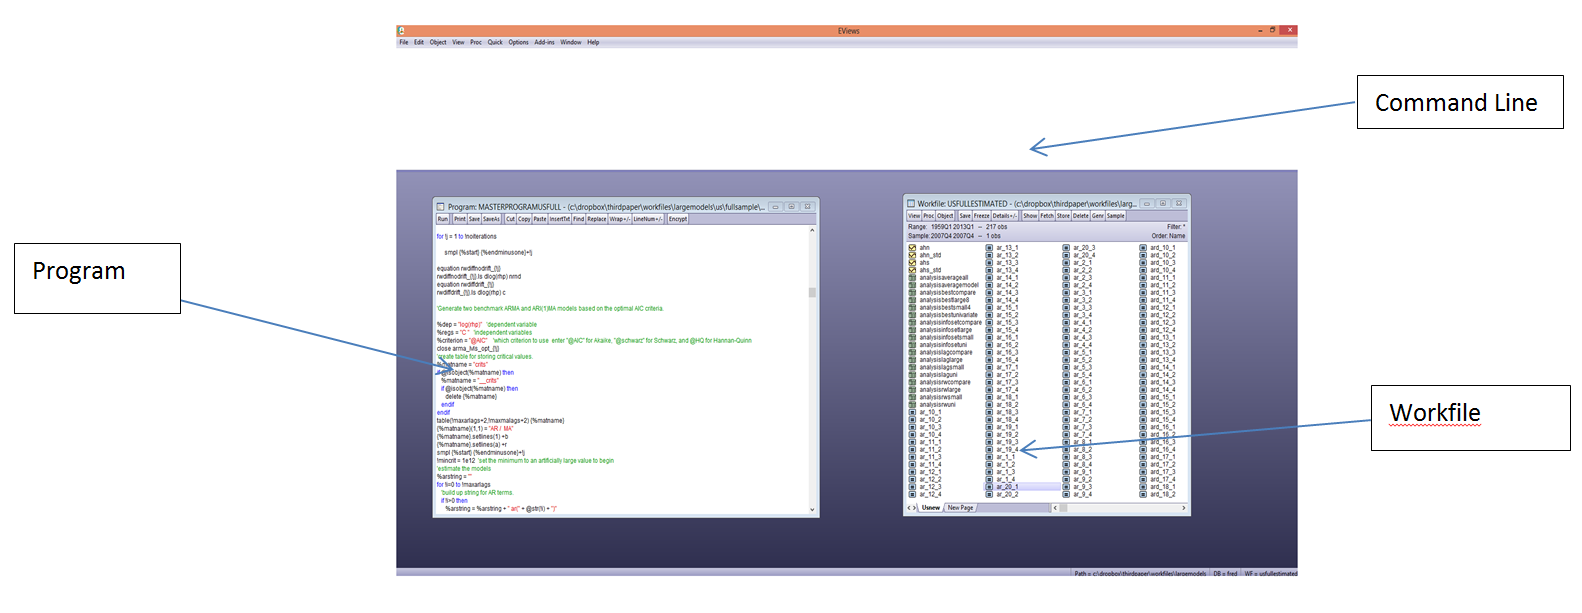
\includegraphics{interface.png}}
\end{figure}
\end{center}
\begin{itemize}
\item Find the program window from File $\rightarrow$ New $\rightarrow$ program.\\[0.1in]
\item Try changing the background colour in your EViews (`Options'$\rightarrow$`General Options'). Have a look at some of the other options there too.
\end{itemize}
}

%TYPES OF WORKFILE
%\item Lets open our first workfile: \texttt{wfcreate u 1}.\\[0.1in]

\frame{\frametitle{Workfile Structures}
\begin{itemize} 
\item One thing to be aware of at this stage is the different types of \textbf{workfile}:
\end{itemize}
\begin{center}
\begin{figure}
    \scalebox{.3}{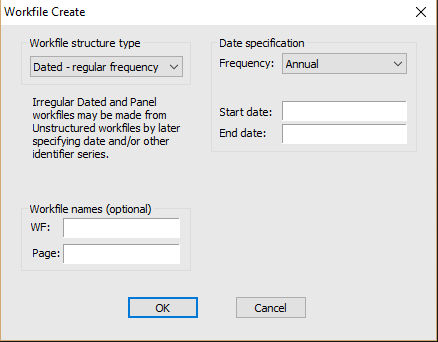
\includegraphics{workfiles.png}}
\end{figure}
\end{center}
\begin{itemize}
\item Your main choices are: \texttt{Unstructured/Undated}, \texttt{Dated -- Regular Frequency}, \texttt{Balanced Panel}.\\[0.1in]
\item There are various frequencies available with the latter two.\\[0.1in]
\item Be aware that \texttt{C} and \texttt{resid} will \textbf{always} be present in your workfiles.
\end{itemize}
}

\frame{\frametitle{Object Types}
\begin{itemize} 
\item One thing to be aware of at this stage is the different types of \textbf{object}:
\end{itemize}
\begin{center}
\begin{figure}
    \scalebox{.3}{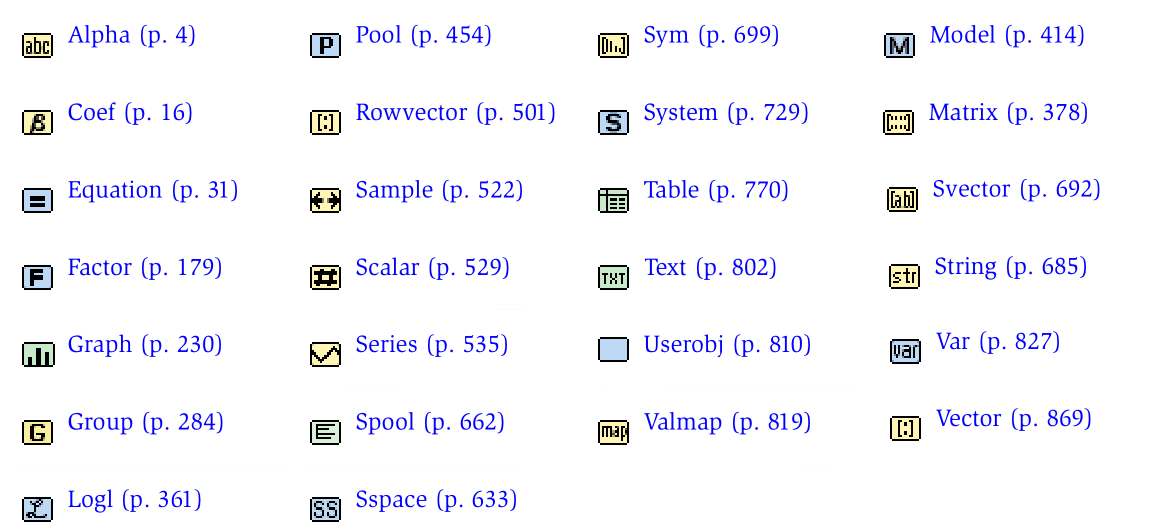
\includegraphics{objects.png}}
\end{figure}
\end{center}
\begin{itemize}
\item Lets create a workfile (\texttt{wfcreate u 1}) and some of the basic objects.\\[0.1in]
\item \small \texttt{`scalar hello = 1'}, \texttt{`vector(5) msc = 5'}, \texttt{`matrix(2,2) students = 10'}.
\end{itemize}
}

\section{Figures}
\subsection{Slide 1}
\frame{\frametitle{Importing and Plotting: Slide 1}
Lets see if we can import some data and replicate this graph:
\begin{figure}
    \scalebox{.095}{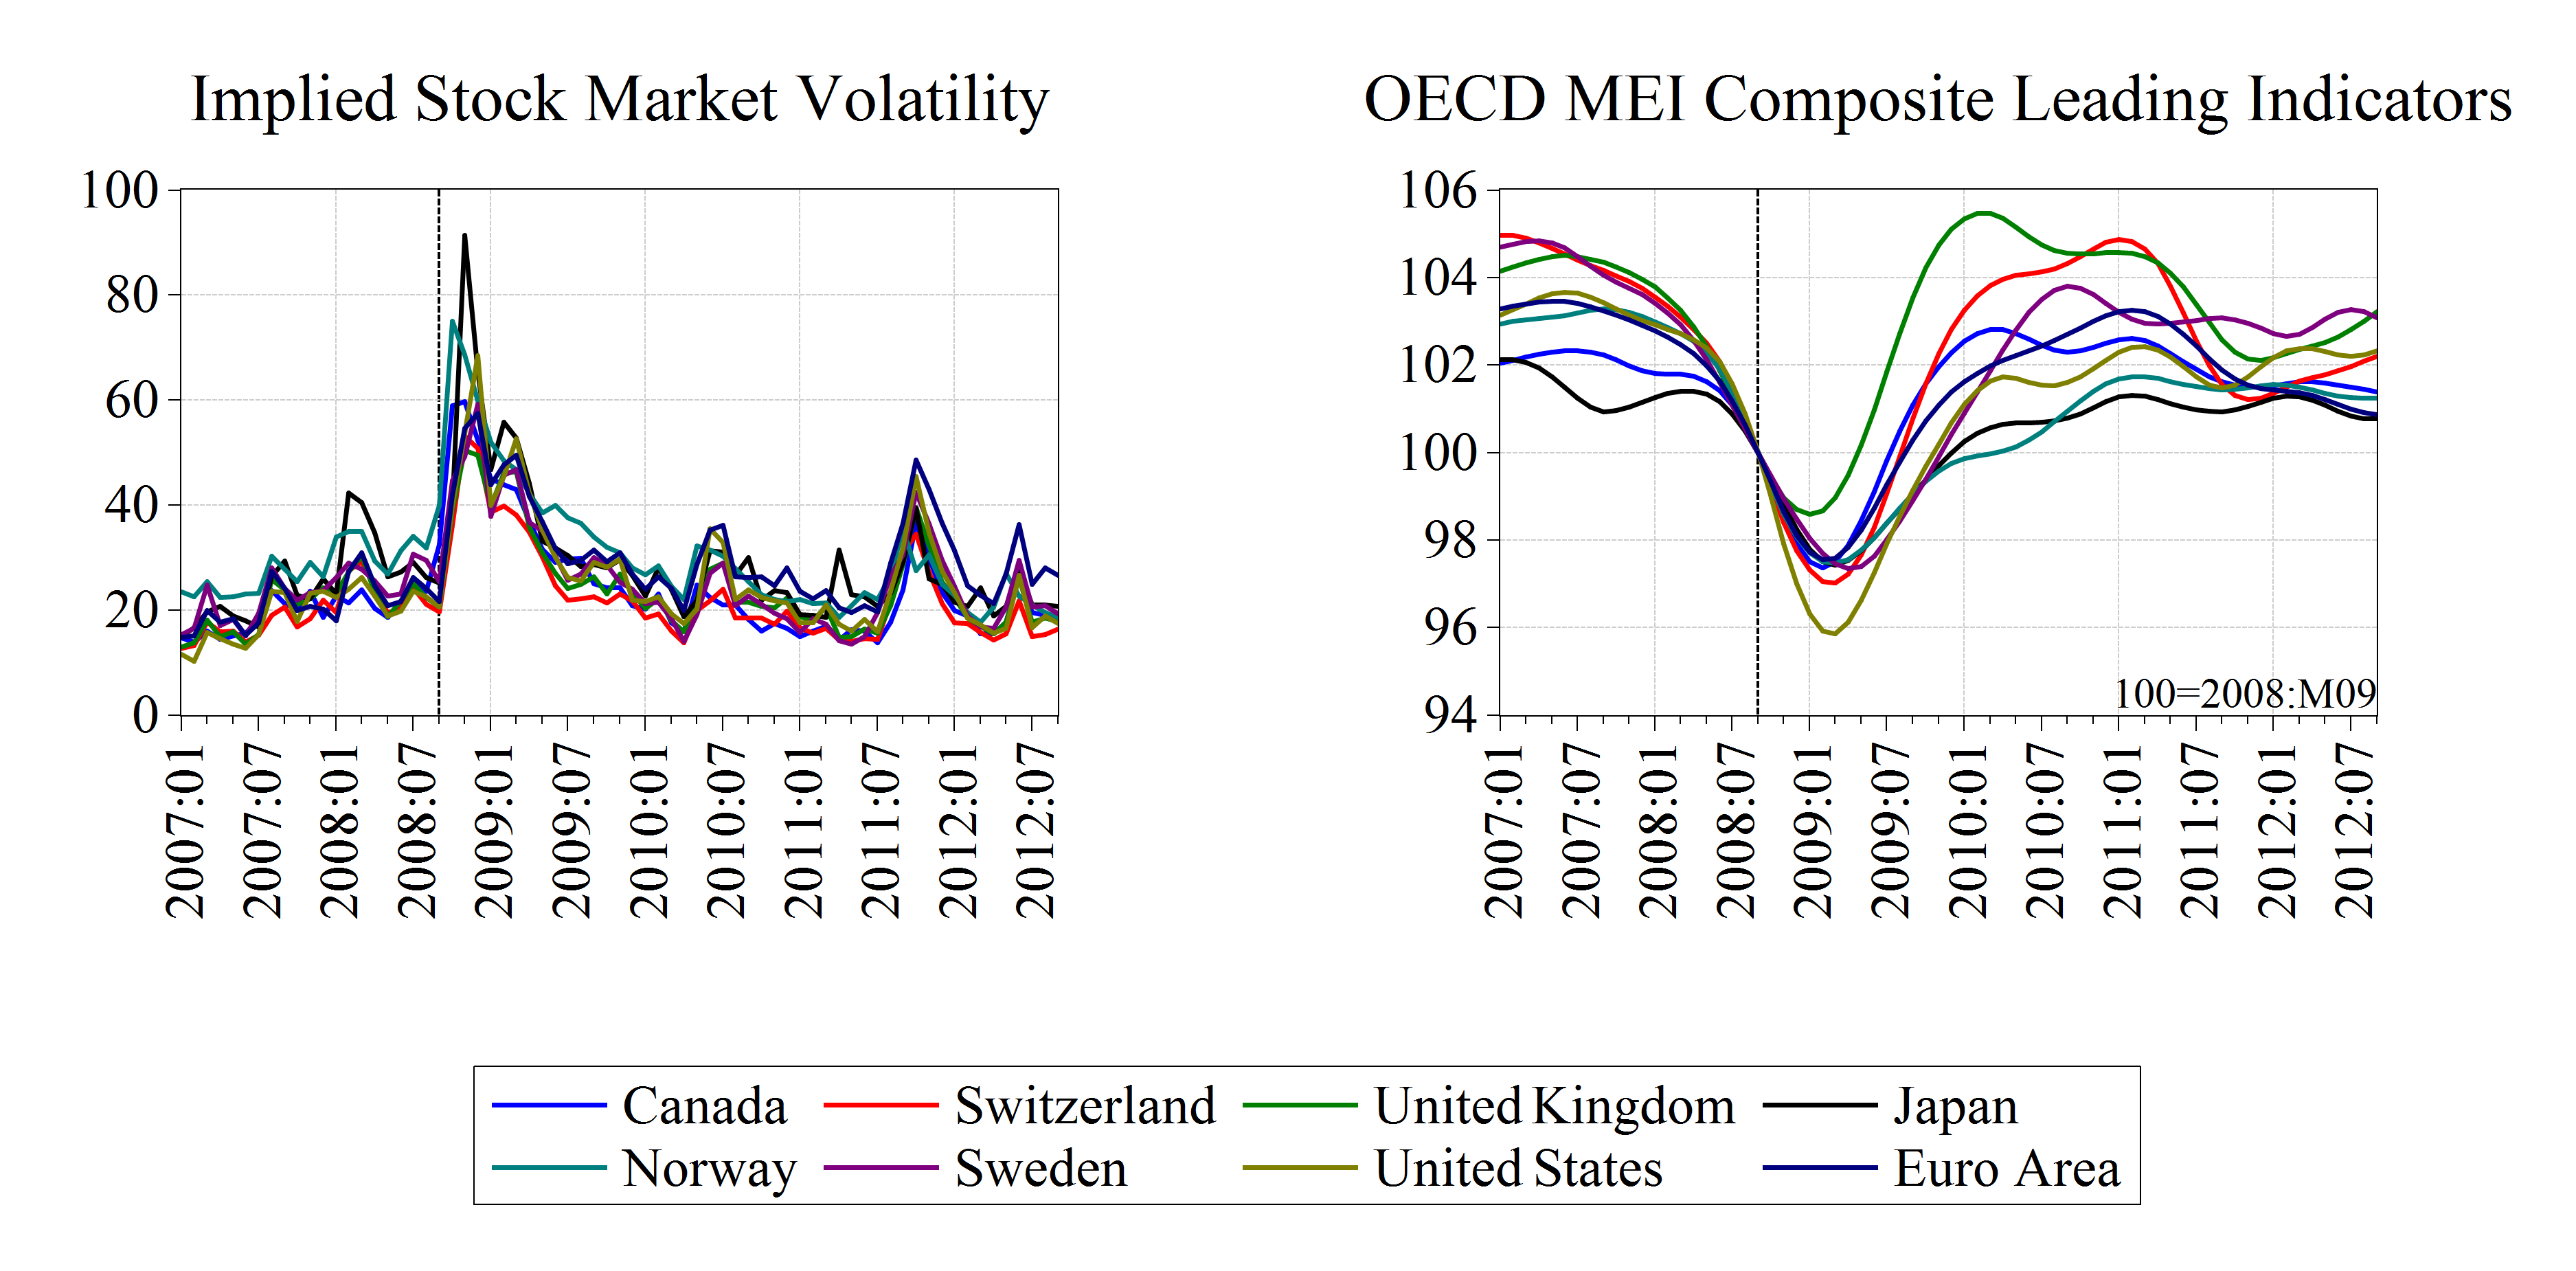
\includegraphics{ivolandcci.png}}
\end{figure}
\begin{itemize}
\item Shows spike in implied (VIX) stock market volatility and fall in confidence indicators following Lehman collapse.\\[0.1in]
\end{itemize}
}

\subsection{Slide 2}
\frame{\frametitle{Importing and Plotting: Slide 2}
\begin{itemize}
%\item Graph (\emph{ivolandcc.png}) should be in your Canvas folder.\\[0.2in]
\item The data used is in \emph{figure1data.xls} which accompanies these slides.\\[0.2in]
\item Note: earlier versions of EViews struggle with .xlsx file extentions.\\[0.2in]
\item To begin, lets open a dated EViews workfile (\emph{.wf}) from the menus:\\
\begin{center} 
{\setlength\itemindent{75pt} File $\rightarrow$ New $\rightarrow$ Workfile $\rightarrow$ Dated $\rightarrow$ 2007M1 - 2012M9}\\
\end{center}
\item Then, to import our data of interest:\\
\begin{center}
{\setlength\itemindent{75pt} File  $\rightarrow$  Import  $\rightarrow$ Import from file $\rightarrow$ Locate \emph{figure1data.xls}}
\end{center}
\end{itemize}
}

%\subsection{Slide 3}
%\frame{\frametitle{Importing and Plotting: Slide 3}
%Note! You can also do this directly from the command line:\\[0.2in]
%\scriptsize
%\color{blue}{\texttt{wfopen C:\textbackslash filepath\textbackslash figure1data.xls range="Sheet1!\$A\$1:\$ag\$70" @freq m 2007m1}}\\[0.3in]
%\normalsize
%\color{black}{You will of course have to change the file path!}\\[0.2in]
%}


\subsection{Slide 4}
\frame{\frametitle{Importing and Plotting: Slide 4}
You should then have something which looks like this:
\begin{figure}
    \scalebox{.35}{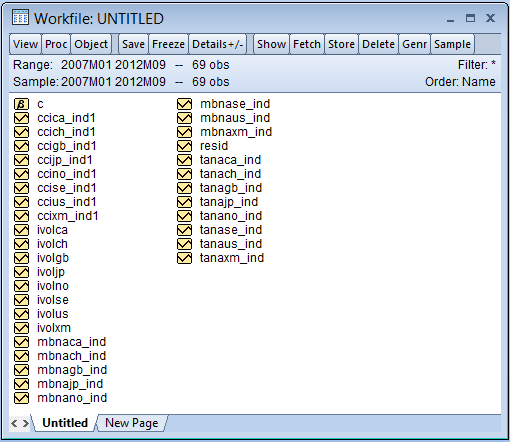
\includegraphics{firstworkfile.png}}
\end{figure}
\begin{itemize}
\item Sample \& range are the same here.\\[0.05in]
\item 69 obs - one per month.\\[0.05in]
\item 32 files from \emph{.xls} plus \texttt{C} and \texttt{resid} which are always present.\\
\end{itemize}
}

\subsection{Slide 5}
\frame{\frametitle{Importing and Plotting: Slide 5}
\begin{itemize}
\item We now want to form the two graphs of interest, one at a time.\\[0.1in]
\item First: Select 8 of your variables of interest (.e.g all the ivol series).
\small
\begin{center}
{\setlength\itemindent{75pt} Right click  $\rightarrow$  Open group $\rightarrow$ Import from file $\rightarrow$ Locate \emph{figure1data.xls}}\\[0.1in]
\end{center}
\normalsize
\item To make a \textbf{graph} \emph{object} out of this \textbf{group} \emph{object}, hit \textbf{Freeze}\\[0.1in]
\item Save both the group and the graph (e.g. as fig1graph/fig1group). \\[0.1in]
\item Open graph, right click, options and adjust the various settings to replicate graph above.\\[0.1in]
\item Repeat for the second graph/data of interest.\\[0.1in]
\end{itemize}
}

\subsection{Slide 6}
\frame{\frametitle{Importing and Plotting: Slide 6}
Important things to pay attention to when plotting these and other graphs:\\[0.1in]
\begin{enumerate}
\item[1.]  Size of the graphs.\\ [0.05in]
\item[2.] The axes.\\ [0.05in]
\item[3.]  Legend.\\ [0.05in]
\item[4.]  Font.\\ [0.05in]
\item[5.]  Gridlines.\\ [0.05in]
\item[6.]  Thickness and colour of lines.\\ [0.05in]
\item[7.] Ideally(!) chose a `pattern' in case your article gets printed in black \& white!\\[0.2in]
\end{enumerate}
You can then save your \texttt{graph object} to disk or copy and paste out (right click) .
}

\subsection{Slide 7}
\frame{\frametitle{Importing and Plotting: Slide 7}
\begin{itemize}
\item You can now `merge' the graphs: Highlight multiple graphs and right click $\rightarrow$ open them together.\\
\item The key features here are `Options on all graphs', which allows you to change multiple settings at once.\\
\item And also, importantly, the `Align and Position' option. \\
%{\setlength\itemindent{25pt} \item  You may have to change this after exporting having considered how it looks in your paper/presentation.}\\
\item You can add a title by:
{\setlength\itemindent{15pt} \item Save your graph as an object called `graphname'}
{\setlength\itemindent{15pt} \item Find the command line, and use command:}\\
\begin{center}
 {\setlength\itemindent{75pt} \color{blue}{\texttt{graphname.addtext(t) "Chart title" }}}
\end{center}
\item Now do the same for the other two sets of eight series in the data - the monetary base (MB) and the central bank total assets (TA).
\end{itemize}
}

%\subsection{Slide 8}
%\frame{\frametitle{Importing and Plotting: Slide 8}
%\begin{itemize}
%\item You can also input data directly into EViews.\\[0.1in]
%\item Lets try another example: \\
%{\setlength\itemindent{75pt} Open a new workfile.}\\
%{\setlength\itemindent{75pt} Choose an undated/unstructured workfile, with 1 observation.}\\
%{\setlength\itemindent{75pt} Now choose Quick $\rightarrow$ Empty Group (edit series).}\\[0.1in]
%\item Now lets input data about `Football League Cup Winners':
%\begin{center}
%\url{http://en.wikipedia.org/wiki/List_of_Football_League_Cup_finals\#Results_by_team}
%\end{center}
%\item Lets input data for the eight teams who've won the league cup the most times.\\
%\item Fill a cell/series and then use the `rename' (right click) function.\\
%\end{itemize}
%}

%\subsection{Slide 9}
%\frame{\frametitle{Importing and Plotting: Slide 9}
%You should now have something which looks like this:\\[0.05in]
%\begin{figure}
%    \scalebox{.4}{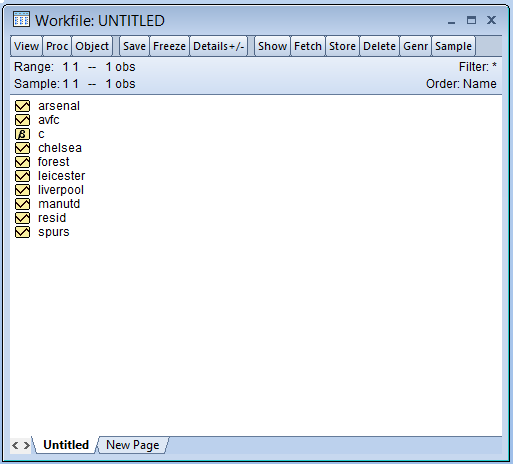
\includegraphics{leaguecupteams.png}}
%\end{figure}
%}

%\subsection{Slide 10}
%\frame{\frametitle{Importing and Plotting: Slide 10}
%Can you replicate this graph?\\[0.075in]
%\begin{figure}
%    \scalebox{.12}{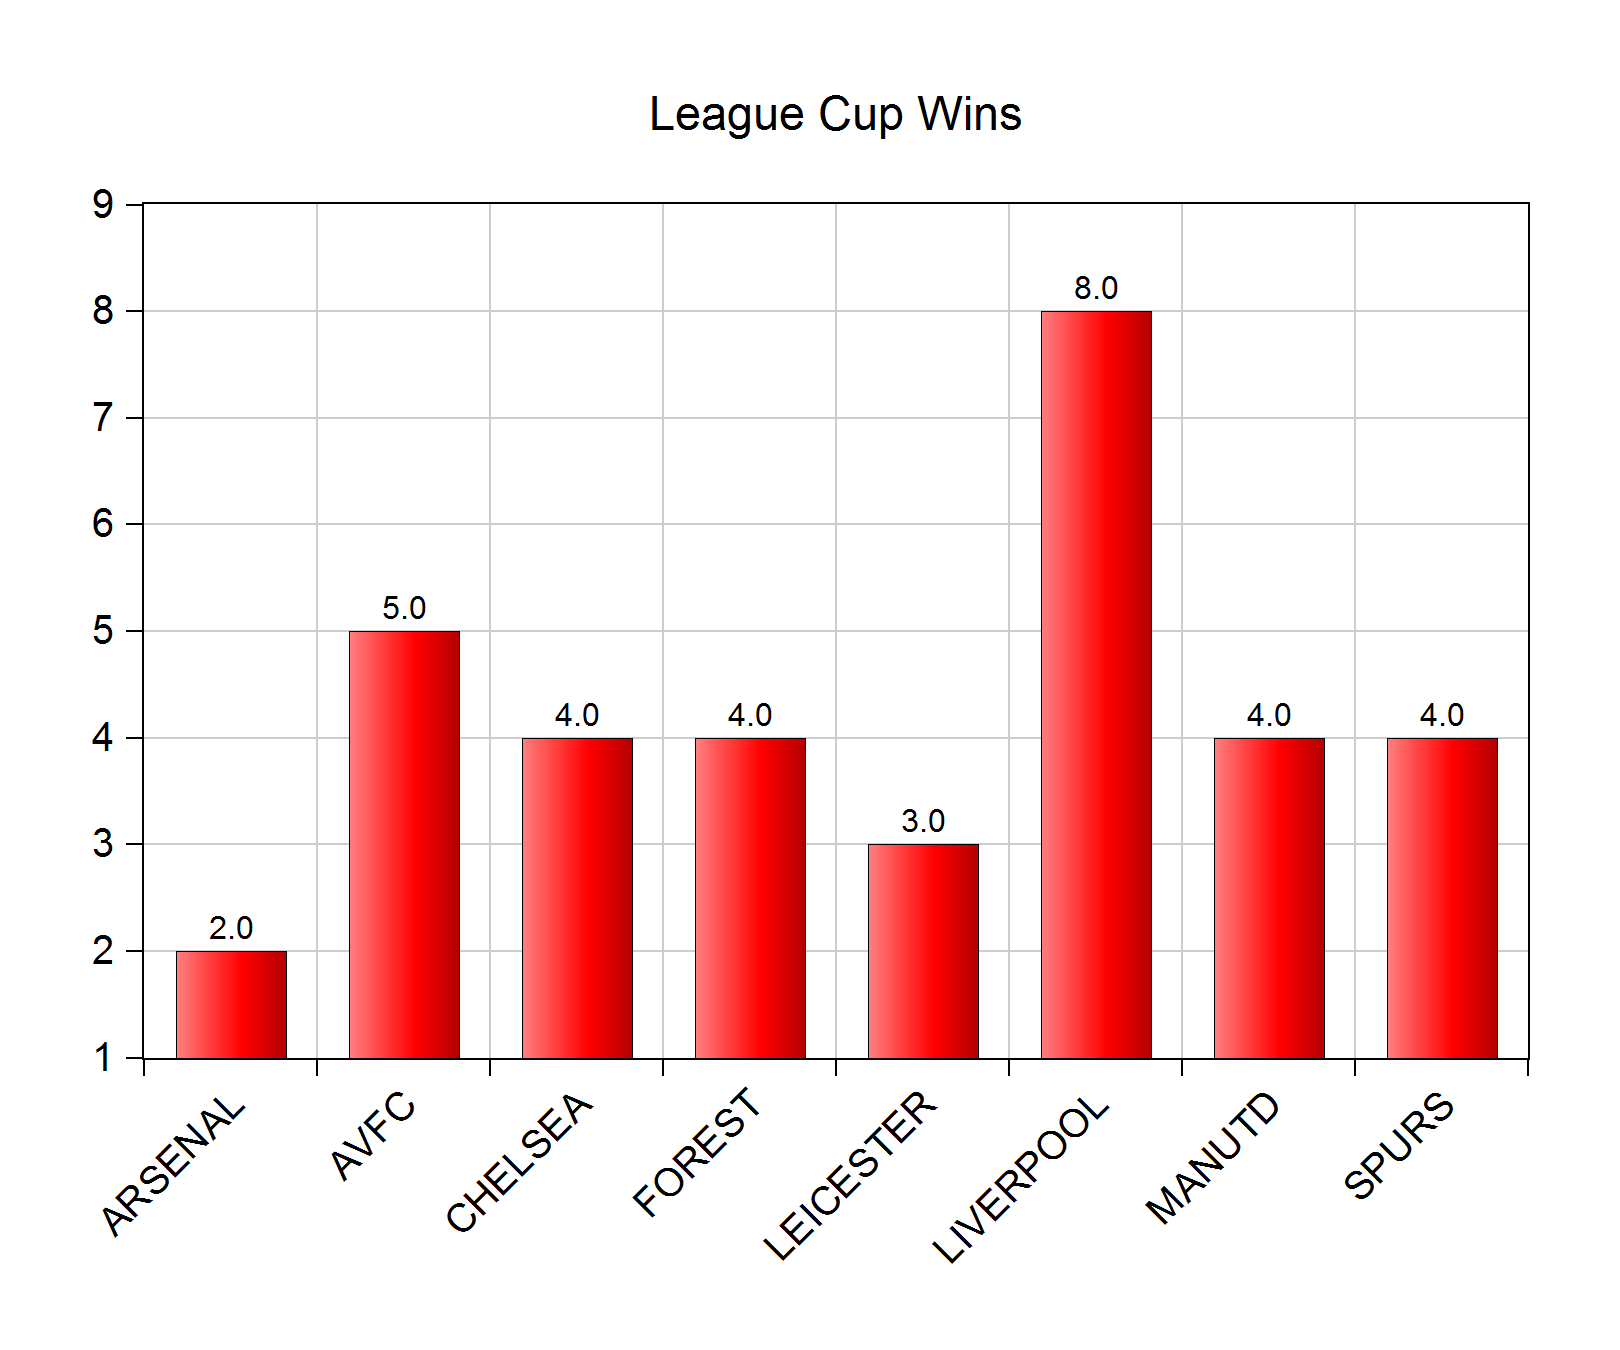
\includegraphics{leaguecupwins.png}}
%\end{figure}
%\begin{itemize}
%\item The key is to specify `Graph data: Mean'\\[0.05in]
%\item Also: note - fill area is `red'\\[0.05in]
%\item 3D Rounded bars, with `label above bar'.\\[0.05in]
%\end{itemize}
%}


\section{Data(bases)}
\subsection{Slide 1}
\frame{\frametitle{Data, Databases and Transformations: Slide 1}
\begin{itemize}
\item Next we introduce an overlooked function - the database.\\[0.1in]
\item One is FRED: \color{red}{F}\color{black}{ederal} \color{red}{R}\color{black}{eserve} \color{red}{E}\color{black}{conomic} \color{red}{D}\color{black}{atabase}.\\[0.1in]
\item FRED is one potential source of data for your dissertation.\\[0.1in]
\item It provides 386,000 US and international time series.\\[0.1in]
\item File  Open $\rightarrow$ Database $\rightarrow$ FRED. Find (`EasyQuery') \& download `gdp' (`WHERE name matches:'), `pcec', `gdpdef' and `permit24nsa'.\\[0.1in]
\item Export to a new workfile, which should then look like this:\\
\end{itemize}
\begin{figure}
    \scalebox{.105}{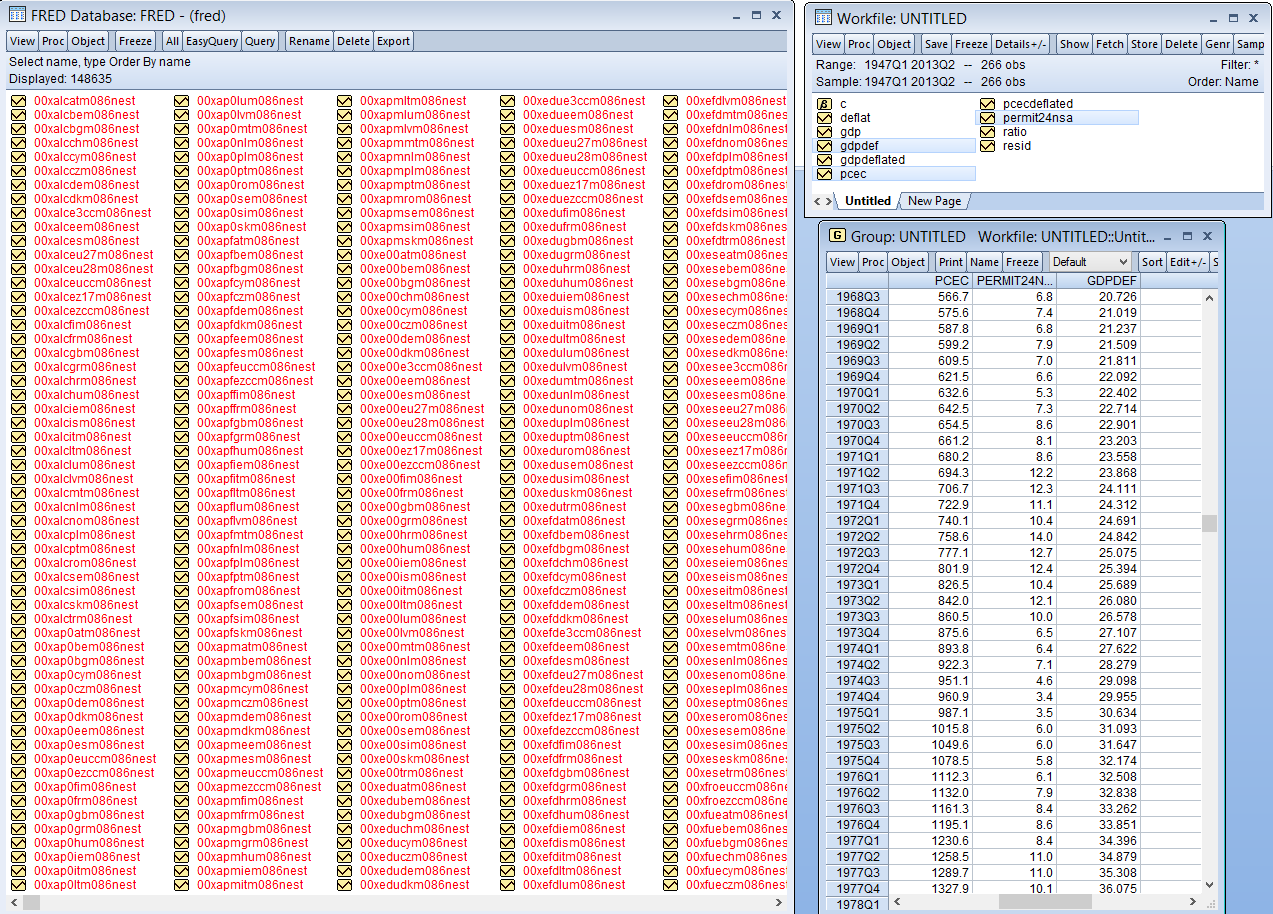
\includegraphics{gdppcecgdpdef.png}}
\end{figure}
}

\subsection{Slide 2}
\frame{\frametitle{Data, Databases and Transformations: Slide 2}
\begin{itemize}
\item First, lets learn about using the command line some more - using deflating as an example.\\[0.2in]
\item Lets create the `decimal form' of our deflater with the command `genr' (generate new series):\\
\begin{center}
\color{blue}{\texttt{genr deflater = gdpdef/100}}\\[0.2in]
\end{center}
\item To deflate GDP and PCEC:\\[0.1IN]
\begin{center}
\color{blue}{\texttt{genr realgdp = gdp/deflater}}\\[0.05in]
\color{blue}{\texttt{genr realpcec = pcec/deflater}}\\[0.05in]
\end{center}
\end{itemize}
}

\subsection{Slide 3}
\frame{\frametitle{Data, Databases and Transformations: Slide 3}
\begin{itemize}
\item Maybe we want to consider the ratio of real consumption to GDP?\\[0.05in]
\begin{center}
\color{blue}{\texttt{genr ratio = realpcec/realgdp}}\\[0.1in]
\end{center}
\item Maybe you want to consider this visually...\\
\begin{figure}
    \scalebox{.175}{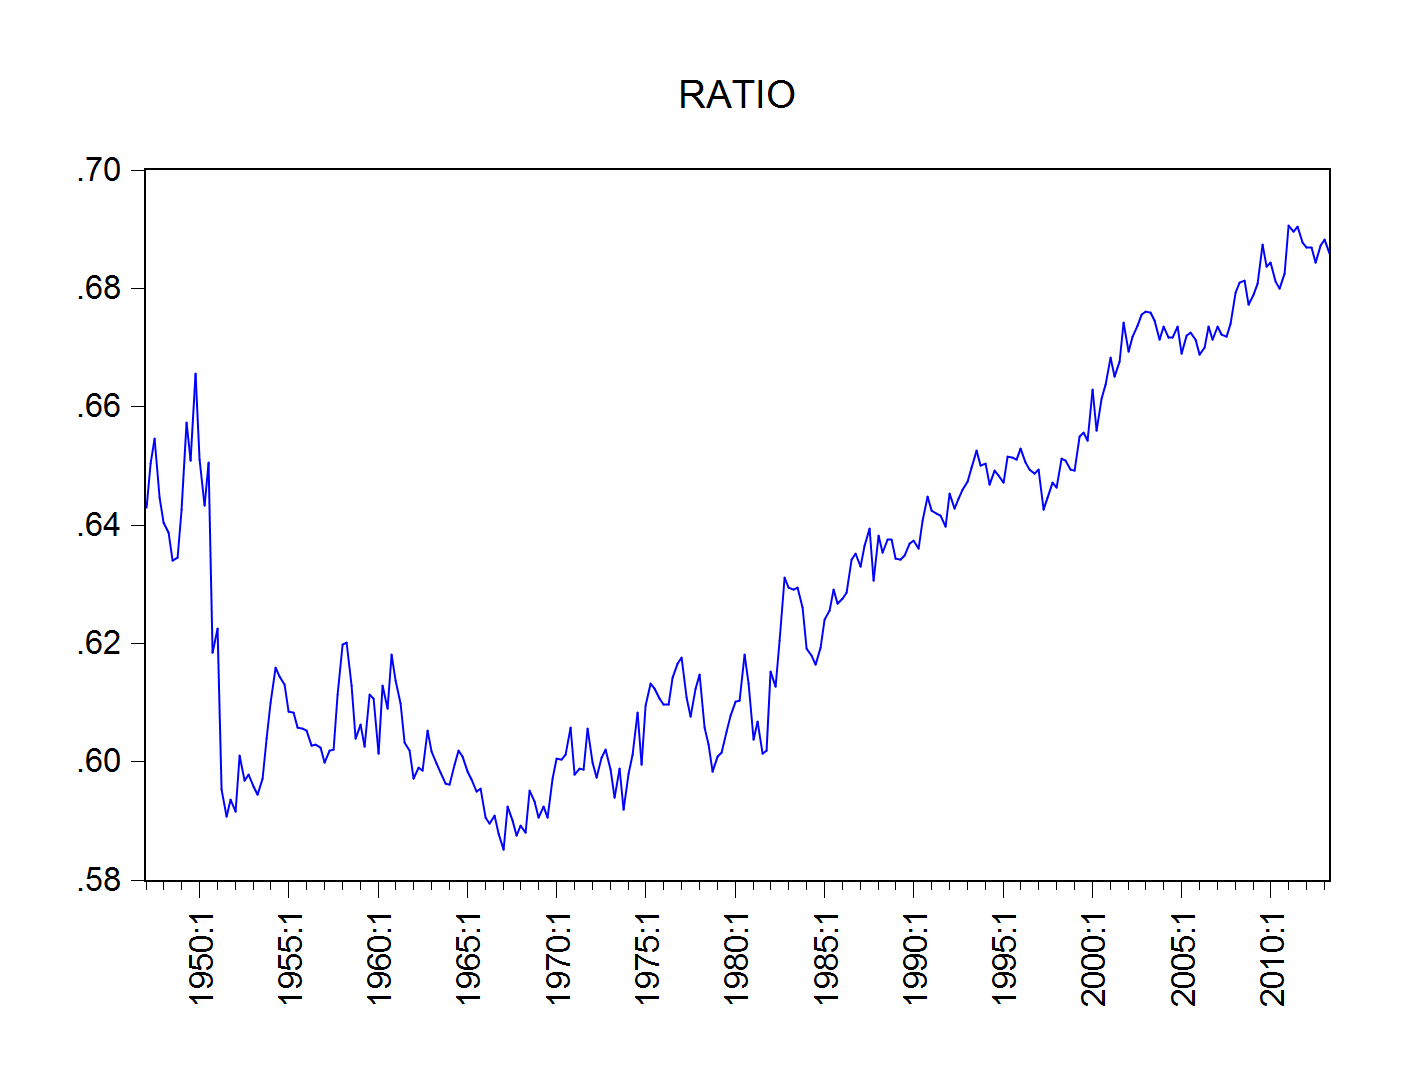
\includegraphics{ratio.png}}
\end{figure}
\end{itemize}
}

\subsection{Slide 4}
\frame{\frametitle{Data, Databases and Transformations: Slide 4}
\begin{itemize}
\item If we want to work with differenced data, we can use the command line:\\
\begin{center}
\color{blue}{\texttt{genr drealgdp = d(realgdp)}}
\end{center}
\item If we want to work with data in logarithms, we can use the command line:\\
\begin{center}
\color{blue}\texttt{{genr lrealgdp = log(realgdp)}}
\end{center}
\item If we want to work with data in first differenced logarithms, we can use the command line:\\
\begin{center}
\color{blue}\texttt{{genr dlrealgdp = dlog(realgdp)}}
\end{center}
\end{itemize}
}

\subsection{Slide 5}
\frame{\frametitle{Data, Databases and Transformations: Slide 5}
\begin{itemize}
\item Next, we will consider seasonal adjustment.\\[0.1in]
\item Open the series on housing permits granted (permit24nsa)\\[0.1in]
\item Proc $\rightarrow$ Seasonal adjustment $\rightarrow$ Census X-13.\\[0.1in]
\item New (adjusted) series should appear as `permit24nsa\_d11'.\\[0.1in]
\item You can also generate this from the command line with:\\
\begin{center}
\color{blue}\texttt{{seriesname.x13}}
\end{center}
\end{itemize}
}

\subsection{Slide 6}
\frame{\frametitle{Data, Databases and Transformations: Slide 6}
\begin{itemize}
\item The adjustment procedure can be seen clearly by plotting both the original and the \_d11 series:\\
\begin{figure}
    \scalebox{.15}{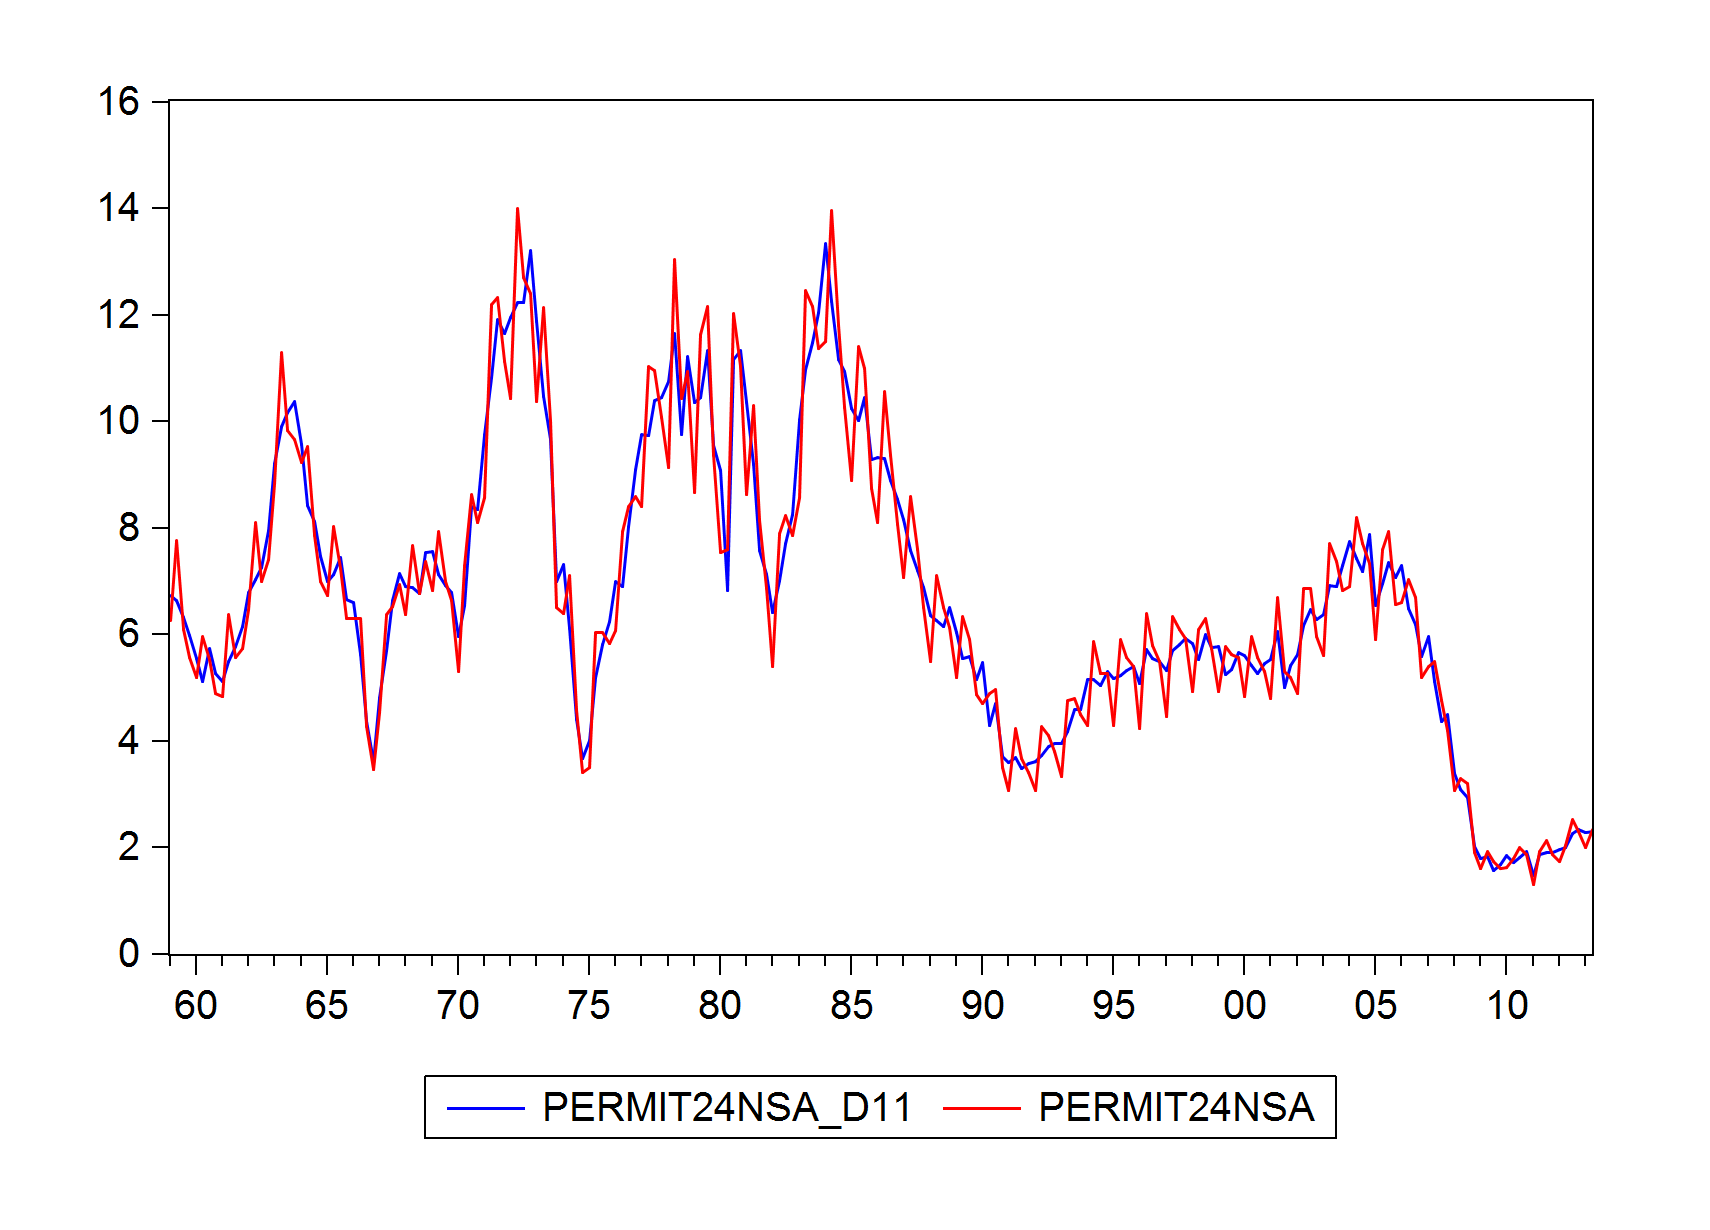
\includegraphics{seasonaladjustment.png}}
\end{figure}
\item However, many series will come `pre-adjusted'.\\[0.2in]
\end{itemize}
}


\subsection{Slide 7}
\frame{\frametitle{Data, Databases and Transformations: Slide 7}
\begin{itemize}
\item This puts series into a group, and then adjusts all the series in a group.\\
\end{itemize}
\begin{shaded}
\begin{center}
\texttt{
\color{black}
\footnotesize
\noindent
wfcreate q 1975q1 2000q1\\
genr x = 5+@trend+5*@nrnd\\
genr y = 5+@trend+5*@nrnd\\
genr z = 5+@trend+5*@nrnd\\
\%adjgroup = "x y z"\\
group seasadjust \{\%adjgroup\}\\
\color{blue}for \color{black} !i=1 to seasadjust.@count\\
\indent   \%name = seasadjust.@seriesname(!i)\\
\indent   \{\%name\}.x12\\
\color{blue}next\color{black}}\\
\normalsize
\color{black}
\end{center}
\end{shaded}
\begin{itemize}
\item To write/use such a program: New $\rightarrow$ Program $\rightarrow$ Run.\\[0.1in]
\item This program introduces more advanced topics which we'll cover later.\\
\end{itemize}
}

\section{Add-ins}
\subsection{Slide 1}
\frame{\frametitle{EViews Add-ins: Slide 1}
\footnotesize
\begin{center}
(keep your seasonally adjusted workfile (\emph{.wf}) open - we will use it again shortly)\\[0.2in]
\end{center}
\normalsize
\begin{itemize}
\item A vital feature of EViews are the `Add-ins': customizable programs which look and feel like built-in procedures.\\[0.1in]
\item They use the standard EViews command/menu and object interface.\\[0.1in]
\item Written by both EViews staff (e.g. the BVAR add-in) and also by the experienced EViews enthusiasts (e.g. my StatFact and MacroTrans addins)\\[0.1in]
\item Students of EViews can also write their own add-ins (a more advanced topic which we will not cover).\\[0.1in]
\end{itemize}
}

\subsection{Slide 2}
\frame{\frametitle{EViews Add-ins: Slide 2}
\begin{itemize}
\item For a full list of add-ins, please visit:\\
\begin{center}
\url{www.eviews.com/addins/addins.shtml}\\[0.1in]
\end{center}
\item There are two ways to install add-ins:\\
\begin{enumerate}
{\setlength\itemindent{5pt} \item[1.] Download .aipz from the URL above}\\[0.1in]
{\setlength\itemindent{5pt} \item[2.] Directly through the EViews client $\rightarrow$ Add-ins tab.}\\[0.1in]
\end{enumerate}
\item Note - these add-ins are only available in EViews 7.1 or later.\\[0.1in]
\end{itemize}
}

\subsection{Slide 3}
\frame{\frametitle{EViews Add-ins: Slide 3}
\begin{itemize}
\item Install one as an example that we can easily utilize with our current workfile - \textbf{RecShade}\\[0.1in]
\item This shades graphs for U.S./Japan recessions, as applicable.\\[0.1in]
\item Install it through either of the two methods outlined on the previous slide.\\[0.1in]
\item To apply it - freeze the graph, and click the `Proc' tab.\\[0.1in]
\item Then scroll down to add-ins and choose add USA Recession Shading (It's U.S. data!)\\[0.1in]
\end{itemize}
}

\subsection{Slide 4}
\frame{\frametitle{EViews Add-ins: Slide 4}
A `RecShade' graph of seasonally adjusted and unadjusted housing starts:
\begin{figure}
    \scalebox{.20}{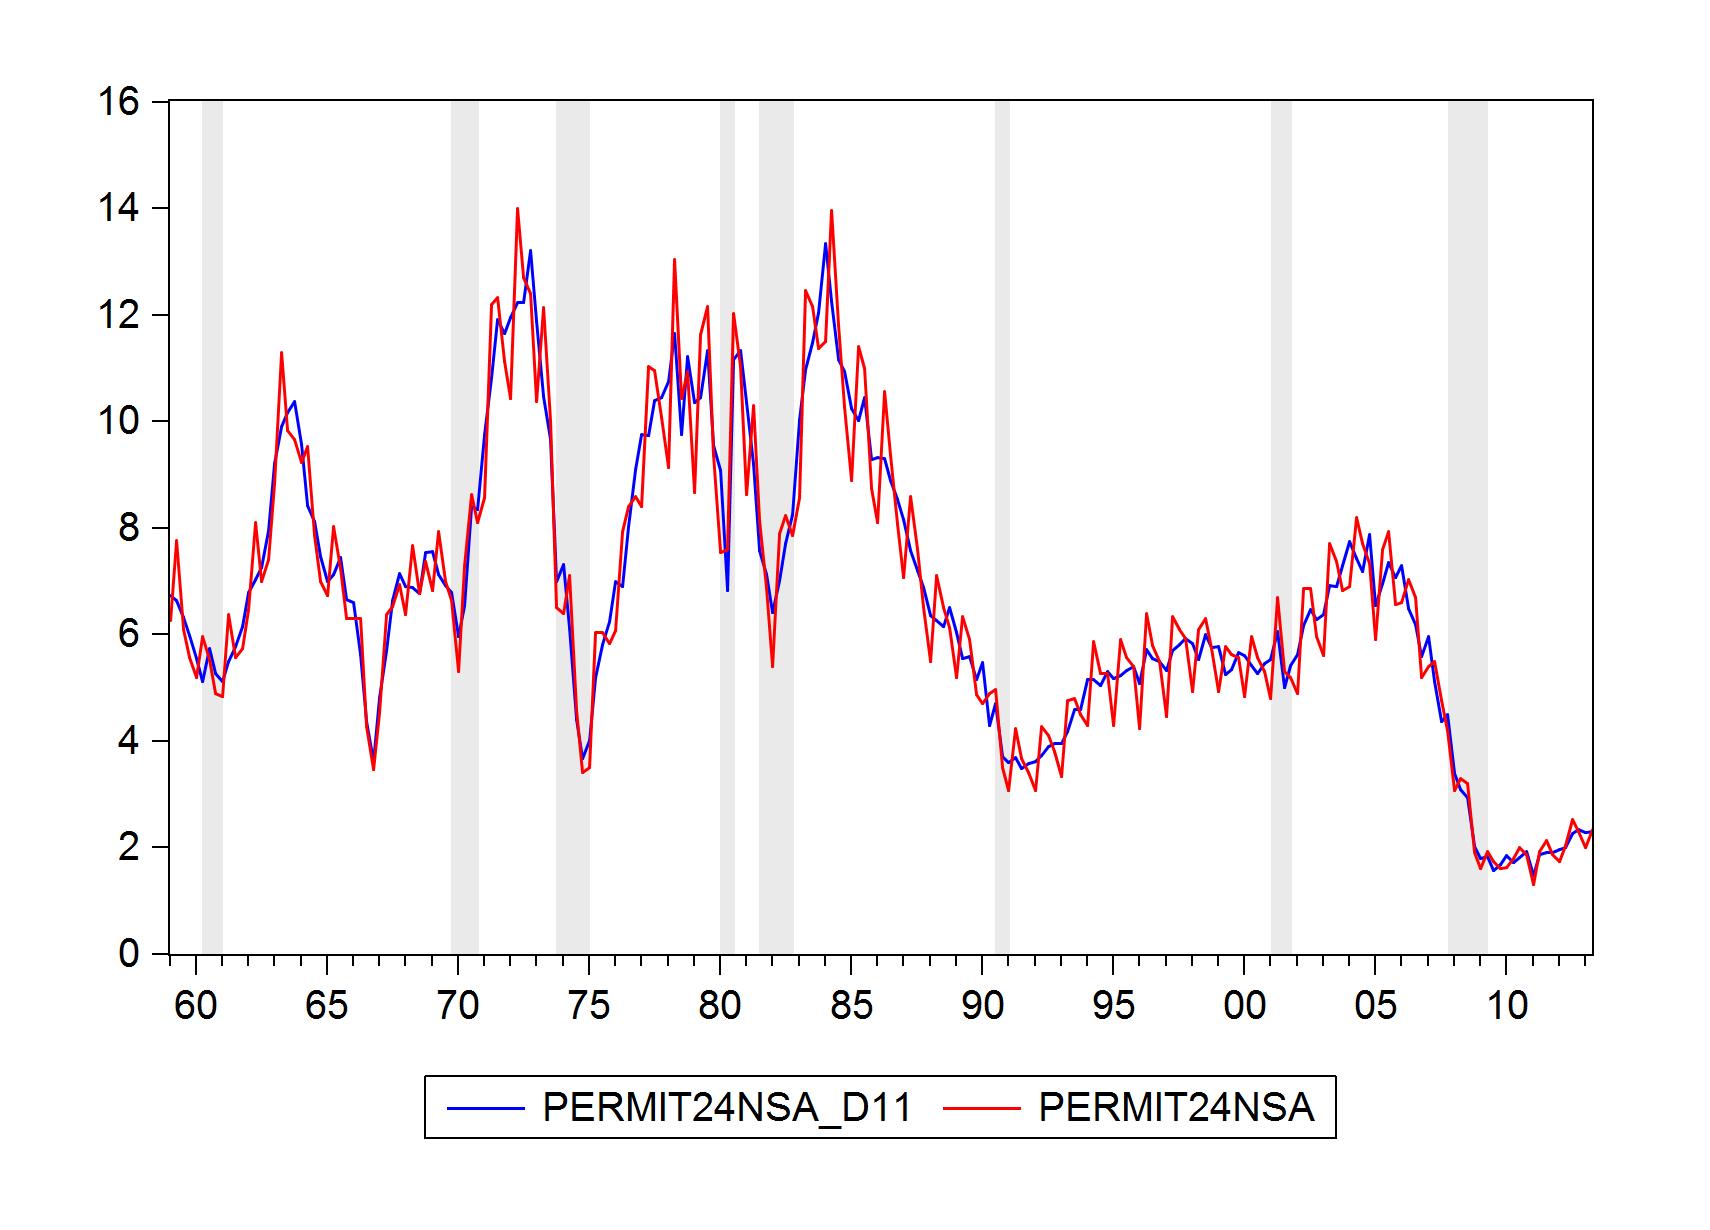
\includegraphics{recshadegraph.png}}
\end{figure}
}

\section{OLS}
\subsection{Slide 1}
\frame{\frametitle{Simple OLS Regression: Slide 1}
\begin{itemize}
\item Lets now consider some simple OLS estimations.\\[0.1in]
\item Begin with the consumption function - a key part of the aggregate expenditure model.\\
\begin{center}
\begin{equation}
{Consumption}_t =\beta_0+\beta_1 {Income}_t + \varepsilon_t
\end{equation}
\end{center}
\item For simplicity, use the simple unadjusted \emph{gdp} and \emph{pcec} series.
\item Then we can obtain estimates of $\hat{\beta_0}$ and $\hat{\beta_1}$ for the consumption function:

\begin{center}
\begin{equation}
\hat{Consumption}=\hat{\beta_0}+\hat{\beta_1{Income}}
\end{equation}
\end{center}	
\vspace{5 mm}
\small
(Try and temporarily ignore any violation of necessary assumptions)
\end{itemize}
}

\subsection{Slide 2}
\frame{\frametitle{Simple OLS Regression: Slide 2}
Three main ways of running this regression in EViews (outside of a batch environment)\\[0.2in]
\begin{enumerate}
\item[1.] Highlight the two series and right click, open as equation, and choose LS estimation.\\[0.1in]
\item[2.] In the workfile window: Object $\rightarrow$ New Object $\rightarrow$ Equation $\rightarrow$ pcec c gdp \\[0.1in]
\item[3.] In the command prompt, type:
\begin{center}
\color{blue}{\texttt{equation eq1.ls pcec gdp c}}\\[0.1in]
\end{center}
\end{enumerate}
}

\subsection{Slide 3}
\frame{\frametitle{Simple OLS Regression: Slide 3}
\begin{itemize}
\item The last option is most informative and you should consider using it most.\\[0.2in]
\item It automatically generates and saves `eq1' object, but the first two don't.\\[0.2in]
\item The `equation' denotes a single equation object. Try as a VAR:\\
\begin{center}
\color{blue}{\texttt{var eq2.ls pcec gdp}}\\[0.1in]
\end{center}
\color{black}
\item Alternatively you can estimate the equation with other methods, e.g. ARCH:
\begin{center}
\color{blue}\texttt{{equation eq3.arch pcec gdp c}}\\[0.1in]
\end{center}
\end{itemize}
}

\subsection{Slide 4}
\frame{\frametitle{Simple OLS Regression: Slide 4}
\vspace{0.2in}
\begin{itemize}
\item From our `eq1', we should get results similar to this:
\end{itemize}
\begin{figure}
    \scalebox{.35}{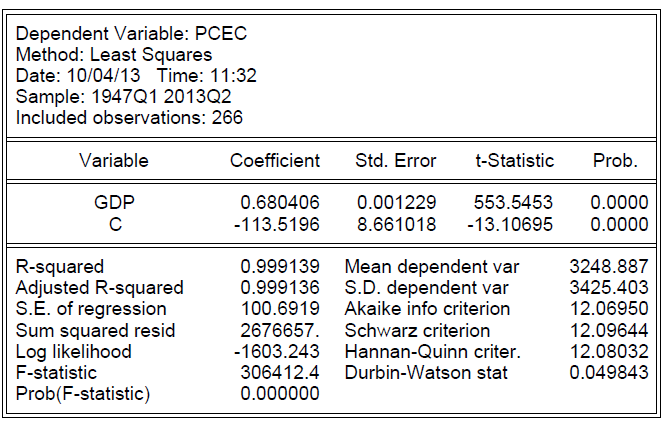
\includegraphics{olsresults}}
\end{figure}
\begin{itemize}
\item From this, we can see that $\hat{\alpha}$=-113.5196 and $\hat{\beta}$=0.680406.\\ [0.1in]
\item Can you figure out why the output differs from these results on the slide?
\end{itemize}
}

\subsection{Slide 5}
\frame{\frametitle{Simple OLS Regression: Slide 5}
\begin{itemize}
\item We also might want to consider a plot of the residuals.
\item Equation: View $\rightarrow$ Actual, Fitted, Residual $\rightarrow$ Actual Fitted Residual Graph
\begin{figure}
    \scalebox{.15}{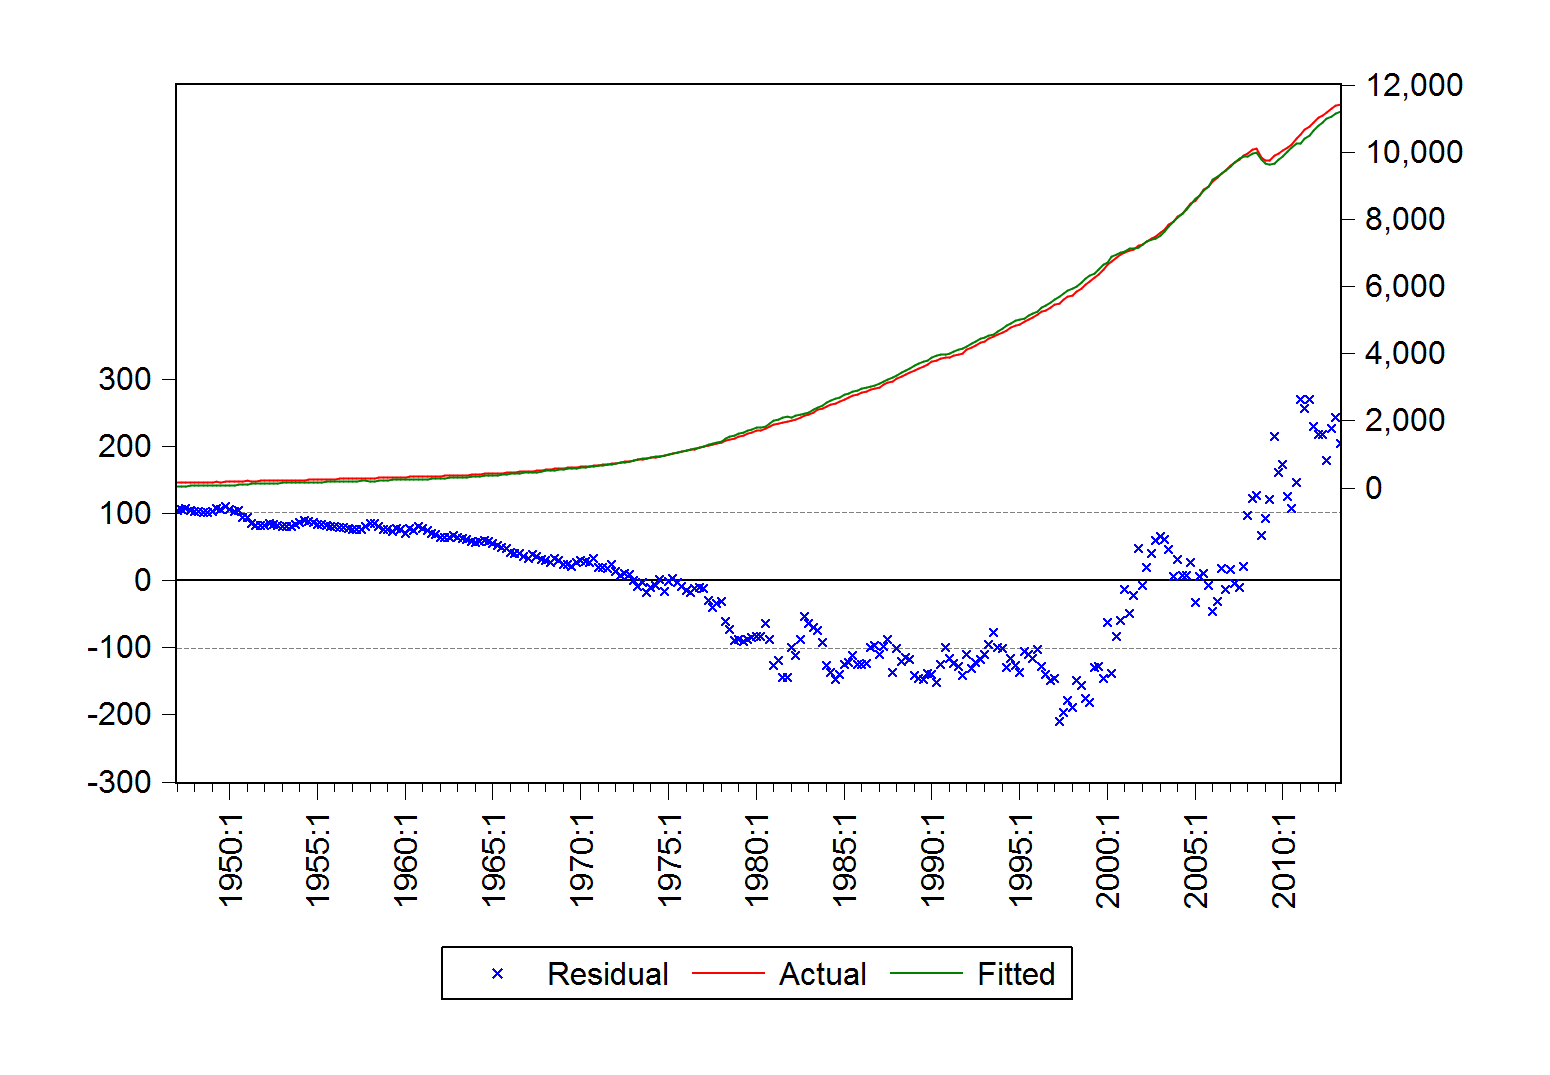
\includegraphics{residualgraph.png}}
\end{figure}
\item Do the residuals look normally distributed?
 \end{itemize}
}


\subsection{Slide 6}
\frame{\frametitle{Simple OLS Regression: Slide 6}
\begin{itemize}
\item From the `View' menu we have a range of different diagnostic tests.\\[0.1in]
\item In particular, we might want a histogram of the residuals to check their non-normality, which also provides the JB statistic and p-value.\\
\end{itemize}
\begin{figure}
    \scalebox{.10}{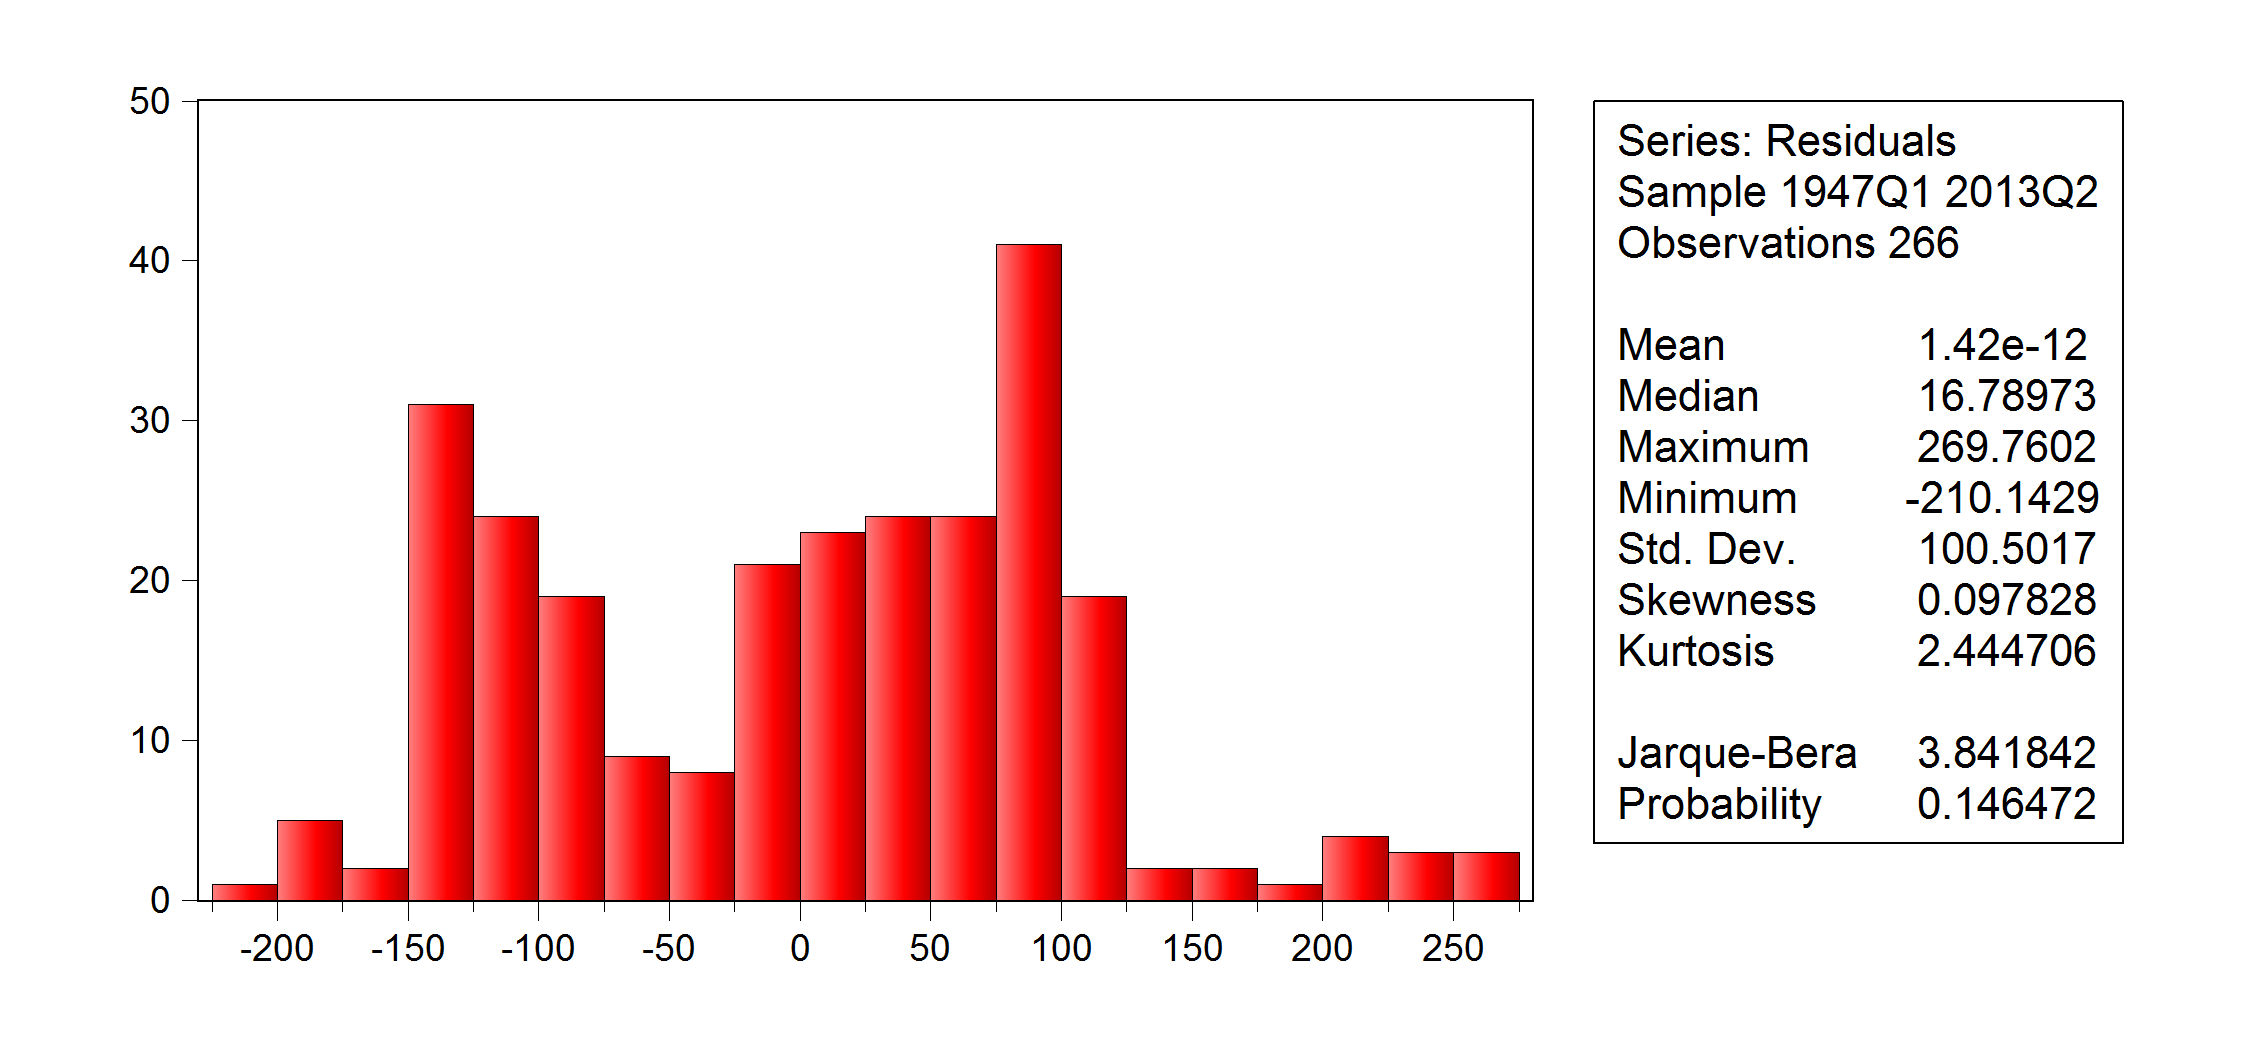
\includegraphics{histogram.png}}
\end{figure}
\begin{itemize}
\item Finally, we might want to plot the estimated function:
\begin{center}
\color{blue}{\texttt{genr pcechat = -113.5196 +0.680406*gdp}}\\[0.1in]
\end{center}
\end{itemize}
}

%\subsection{Slide 7}
%\frame{\frametitle{Simple OLS Regression: Slide 7}
%\begin{itemize}
%\item Getting the basics of running OLS estimations right is very important, so let's try another example.\\[0.1in]
%\item Download the data on food expenditure and income from:\\[0.1in]
%\begin{center}
%\url{www.principlesofeconometrics.com/poe4/data/excel/food.xlsx}
%\end{center}
%\item Create an undated dataset with 40 observations, and run the OLS regression:\\[0.05in]
%\begin{center}
%\color{blue}{ \texttt{equation eq.ls food\_exp c income}}\\[0.1in]
%\end{center}
%\end{itemize}
%}


%\subsection{Slide 8}
%\frame{\frametitle{Simple OLS Regression: Slide 8}
%\begin{itemize}
%\item The results should look something like this:
%\end{itemize}
%\begin{figure}
%    \scalebox{.45}{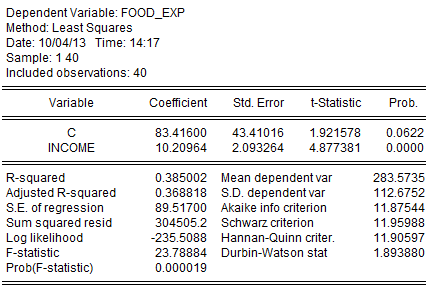
\includegraphics{foodexpresults.png}}
%\end{figure}
%\begin{itemize}
%\item The $t$ and $p$ values correspond to a test of insignificance.
%\end{itemize}
%}

%\subsection{Slide 9}
%\frame{\frametitle{Simple OLS Regression: Slide 9}
%If we wanted to plot a scatter graph of the regression line:\\
%\begin{itemize}
%\item Open the series as group by right clicking on them both (click income first).\\
%\item View $\rightarrow$ Graph $\rightarrow$ Choose scatter $\rightarrow$ Add regression line from the `fit lines' option.\\
%\item To change the axes (as in graph below):\\
%\item Options $\rightarrow$ Axes \& scaling $\rightarrow$ Data scaling $\rightarrow$ left axis scale endpoints $\rightarrow$ User specified $\rightarrow$ Min: %0, Max: 600.\\
%\end{itemize}
%\begin{figure}
%    \scalebox{.10}{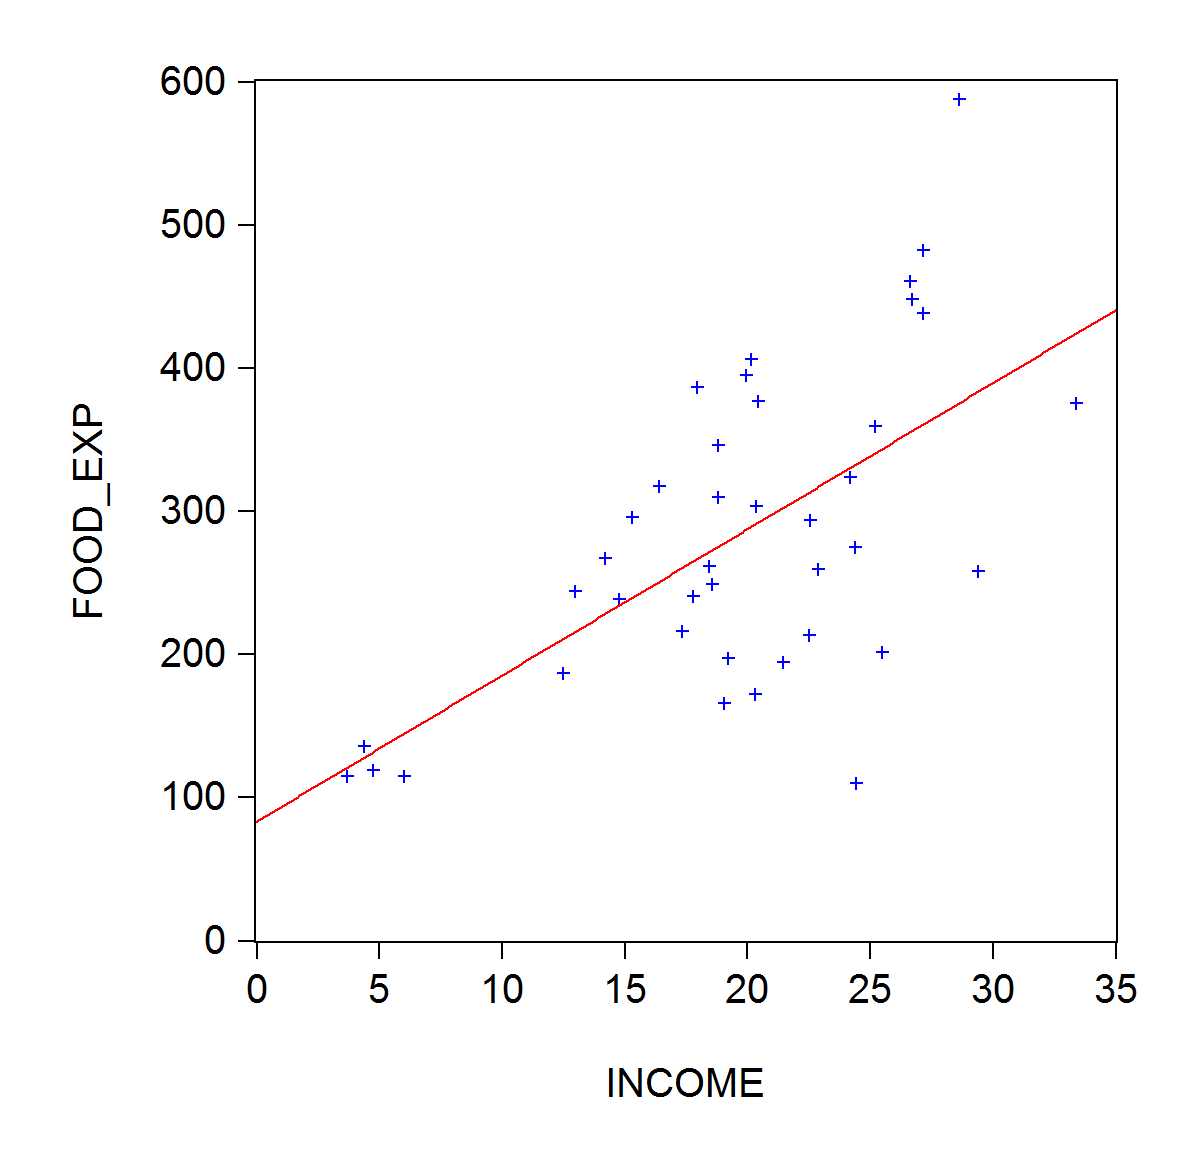
\includegraphics{scatter.png}}
%\end{figure}
%}


%\subsection{Slide 10}
%\frame{\frametitle{Simple OLS Regression: Slide 10}
%\begin{itemize}
%\item We could also run this very simple program:\\[0.2in]
%\begin{shaded}
%\texttt{
%\scriptsize
%\begin{center}
%\noindent wfopen C:\textbackslash <file>\textbackslash food.xls range="Data!\$A\$1:\$B\$41"\\
%equation eq.ls food\_exp c income\\
%scat income food\_exp\\
%\end{center}
%\normalsize
%}
%\end{shaded}
%\end{itemize}
%}

\section{Forecasting}
\subsection{Slide 1}
\frame{\frametitle{An Introduction to Forecasting - Slide 1}
\begin{center}
\emph{'An economist is an expert who will know tomorrow why the things he predicted yesterday didn't happen today.'}\\[0.1in]
\end{center}
\begin{itemize}
\item One of the best features of EViews is the ability of the software to handle the mechanics of producing a forecast.\\[0.1in]
\item It allows the researcher to focus solely on the model specification in order to produce the best forecast.\\[0.1in]
\item Lets return to our housing permits example, and try and forecast PERMIT24NSA.\\[0.1in]
\end{itemize}
}


\subsection{Slide 2}
\frame{\frametitle{An Introduction to Forecasting - Slide 2}
\begin{itemize}
\item Lets model the system as a function of a time trend, lagged growth of itself, and a different constant for each quarter.\\[0.2in]
\item We need to estimate the system before we can forecast it:\\[0.2in]
\begin{center}
\texttt{
\footnotesize{\color{blue}equation forecast1.ls permit24nsa @trend permit24nsa(-1) @expand(@quarter)}}\\[0.2in]
\end{center}
\item Note: @trend is the time trend, the suffix (-1) adds a lagged indenpendant variable, and @expand creates seasonal dummy variables.\\
\end{itemize}
}

\subsection{Slide 3}
\frame{\frametitle{An Introduction to Forecasting - Slide 3}
Generating forecasts is as easy as clicking the 'forecast' button.
\begin{figure}
    \scalebox{.35}{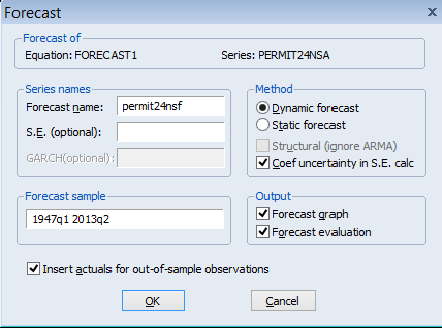
\includegraphics{forecastwindow.png}}
\end{figure}
\begin{itemize}
\item Two important theoretical issues to address at this point.\\[0.1in]
\end{itemize}
}

%\subsection{Slide 4}
%\frame{\frametitle{An Introduction to Forecasting - Slide 4 (Optional)}
%\footnotesize
%\begin{block}{Root Mean Squared Error}{The RMSE is the standard deviation  of the forecast errors.}
%\end{block}
%\begin{block}{Mean Absolute Error}{The MAE is an average of the absolute errors.}
%\end{block}
%\begin{block}{Bias Proportion}{This indicates how the mean of the forecast lies from the actual series}
%\end{block}
%\begin{block}{Variance Proportion}{This indicates how far the actual variance of the forecasts are from the variance of the actual series}
%\end{block}
%\begin{block}{Covariance Proportion}{Measures the remaining unsystematic errors where the Covariance, Variance and Bias proportions add up to one}
%\end{block}
%}


\subsection{Slide 5}
\frame{\frametitle{An Introduction to Forecasting - Slide 5}
\begin{enumerate}
\item[1.] The issues of estimation and forecast samples.\\
\item[2.] The difference between a static and dynamic forecast.\\
\end{enumerate}
\begin{itemize}
\item Always be sure you are estimating your model using information from the correct sample.\\[0.1in]
\item Are you forecasting within sample to consider your model fit?\\[0.1in]
\item Or do you want to forecast out of sample - the unknown future?\\[0.1in]
\item One very common approach is to estimate your model to a certain point in time, then forecast out of sample, and compare the forecast results with that which actually happened.%(artificial history vs artificial future)\\[0.1in]
\end{itemize}
}

\subsection{Slide 6}
\frame{\frametitle{An Introduction to Forecasting - Slide 6}
\begin{itemize} 
\item Another very important distinction is the one between static and dynamic forecasting. From `EViews Illustrated' (Startz (2013)):\\[0.1in]
\begin{enumerate}
\item[1.] \textbf{Static Forecasts}: A static forecast uses the actual values of the explanatory variables in making the forecast. \\ [0.1in]
\item[2.] \textbf{Dynamic Forecasts}: A dynamic forecast uses the forecast value of lagged dependent variables in place of the  actual value of the lagged  dependent variables.\\ [0.1in]
\end{enumerate}
\end{itemize}
}

\subsection{Slide 7}
\frame{\frametitle{An Introduction to Forecasting - Slide 7}
\begin{itemize} 
\item Lets show an example of the effect of using seasonal dummies and while using in-and-out of samples correctly.\\[0.1in]
\item We're going to use 3 distinct, different sample periods.\\[0.1in]
\item It'll give u some good practice using the command line/batch interfaces.\\[0.1in]
\item As you can see below: we are going to estimate our model up until 2005q4. We are then going to use this model to forecast `out of sampple' for the remainder of the period.\\[0.1in]
\item We'll estimate two models: \texttt{modelyesseasonal} and \texttt{modelnoseasonal}.\\[0.1in]
\item \textbf{An optional homework:} Seasonally adjust the series and then repeat the exercise. How do your results differ?
\end{itemize}
}

\subsection{Slide 8}
\frame{\frametitle{An Introduction to Forecasting - Slide 8}
\scriptsize
\texttt{
\hspace{9mm}dbopen(type=fred, server=api.stlouisfed.org/fred, type=fredv1)\\
\hspace{10mm}wfcreate m 1959M01 2016M05\\
\hspace{10mm}fetch(d=fred) permit24nsa\\
\hspace{10mm}smpl @first 2005q4\\
\hspace{10mm}equation modelyesseasonal.ls permit24nsa @trend permit24nsa(-1) @expand(@quarter)\\
\hspace{10mm}smpl 2006q1 @last\\
\hspace{10mm}forecast modelyesseasonal\_f\\
\hspace{10mm}smpl @first 2005q4\\
\hspace{10mm}equation modelnoseasonal.ls permit24nsa @trend permit24nsa(-1)\\
\hspace{10mm}smpl 2006q1 @last\\
\hspace{10mm}forecast modelnoseasonal\_f\\
\hspace{10mm}smpl @all\\
\hspace{10mm}plot permit24nsa modelyesseasonal\_f modelnoseasonal\_f\\[.3in]
}
\normalsize
As can be shown, fit creates a static forecast and forecast creates dynamic forecasts. Plot is the familiar command from earlier slides, which produces the graph on the following slide.
}

\subsection{Slide 9}
\frame{\frametitle{An Introduction to Forecasting - Slide 9}
\begin{figure}
    \scalebox{.25}{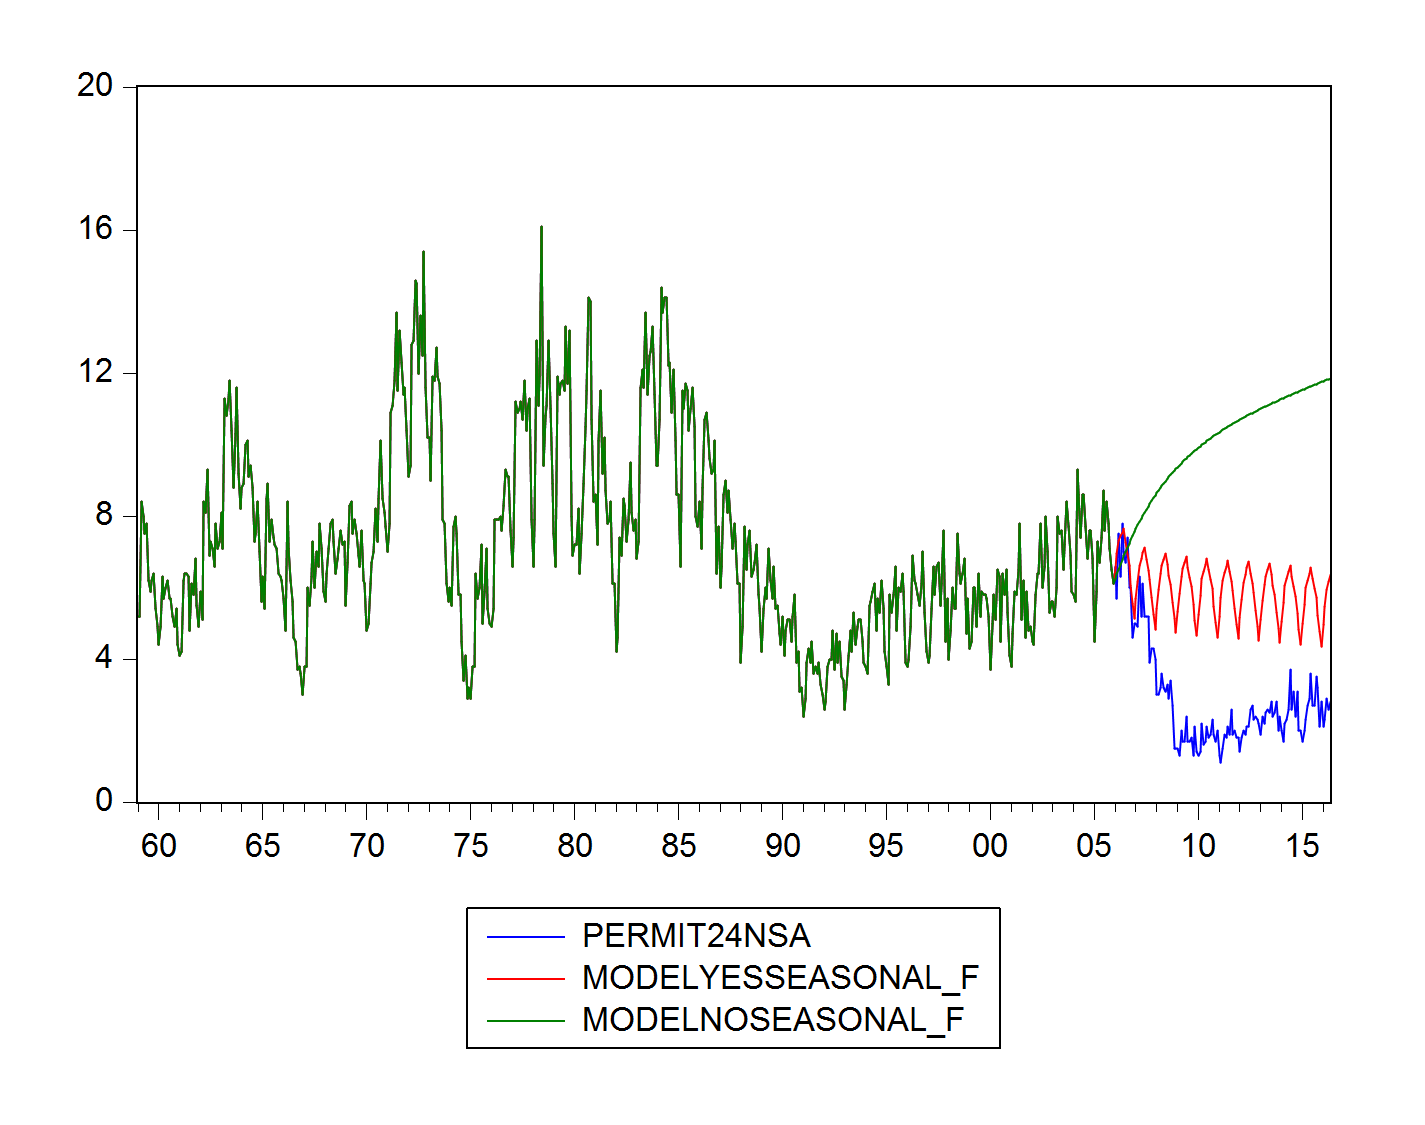
\includegraphics{forecastgraph.png}}
\end{figure}
}

%\subsection{Slide 10}
%\frame{\frametitle{An Introduction to Forecasting - Slide 10}
%What can we tell about these forecasts?
%\begin{itemize}
%\item They appear to forecast relatively well, especially during the first half of the forecast sample until around 2003.\\[0.1in]
%\item As we would obviously expect the static model more closely tracks the actual series.\\[0.1in]
%\item The model appears to over-estimate the seasonal element of the estimation.
%\item The dynamic model is unable to forecast the run-up and crash in the housing market between 2002-2009.\\[0.1in]
%\end{itemize}
%}



\section{VAR Models}
\subsection{Slide 1}
\frame{\frametitle{VAR and VECM Models - Slide 1}

\begin{itemize}
\item \small{Download `wgmacro.wf': \color{blue}{\texttt{\url{http://www.eviews.com/EViews8/data/wgmacro.wf1}}}}\\[0.1in]
\item \color{black} The dataset is from a well established postgraduate textbook, and contains information on income, investment and consumption (and their first differenced logarithms (\texttt{dl} -- just as in our examples above)).\\[0.1in]
\item \color{black} Lets see what this data looks like:
\begin{figure}
\caption{Data from Lutkepol (2007)}
    \scalebox{.225}{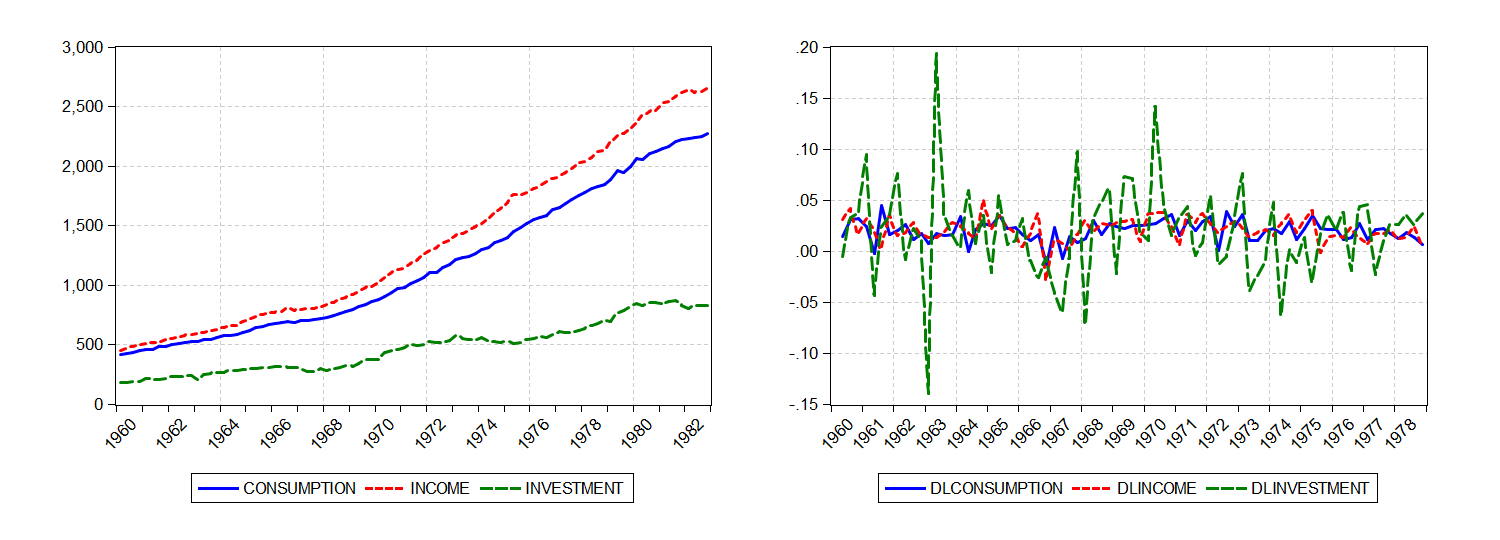
\includegraphics{lutkegraph}}
\end{figure}
\end{itemize}
}


\subsection{Slide 2}
\frame{\frametitle{VAR and VECM Models - Slide 2}
\begin{itemize}
\item Unit root tests: open a series: View $\rightarrow$ Unit Root Test \\ [0.1in]
%\item Hopefully you have been taught about the different tests/nulls.\\[0.1in]
\item Below is an example of a standard ADF test (dlinvestment):\\[0.1in]
\begin{figure}
\caption{An Example ADF test}
\vspace{-0.05in}
    \scalebox{.225}{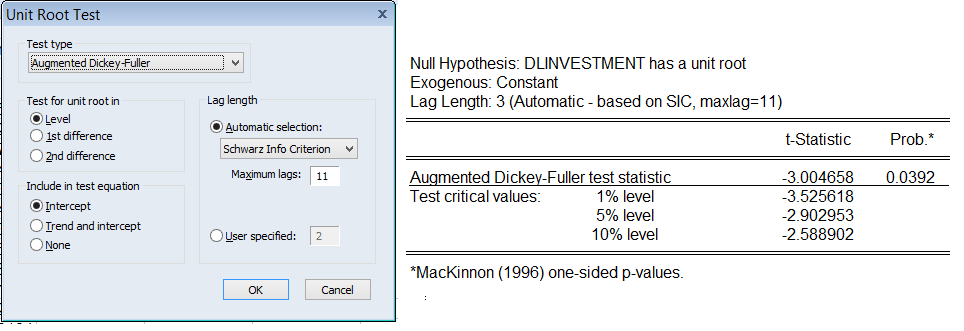
\includegraphics{unitroottest}}
\end{figure}
\item What can we conclude?\\[0.1in]
\item EViews also has several other unit root tests\\
{\setlength\itemindent{15pt} \item And structural unit root add-ins: e.g. Zivot Andrews.}
\end{itemize}
}

\subsection{Slide 3}
\frame{\frametitle{VAR and VECM Models - Slide 3}
There are three ways to open a VAR model (akin to the three ways to open an equation):\\[0.1in]
\begin{enumerate}
\item[1.] Through the command line:\\[0.01in]
\footnotesize
\color{blue}
\begin{center}
\texttt{var myfirstvar.ls 1 2 dlconsumption dlinvestment dlincome}\\[0.1in]
\end{center}
\color{black}
\normalsize
\item[2.] Hold shift and click the three series in the workfile. Right click and select `Open $\rightarrow$ as VAR$\hdots$' \\[0.1in]
\item[3.] Through the menus: Object $\rightarrow$ New Object $\rightarrow$ VAR \\[0.1in]
\end{enumerate}
All three methods will give you the same estimation (try this out!).
}

\subsection{Slide 4}
\frame{\frametitle{VAR and VECM Models - Slide 4}
To determine the appropriate lag length:
\begin{itemize}
\item As a rule of thumb, people can use:
{\setlength\itemindent{15pt} \item 12 lags for monthly data}
{\setlength\itemindent{15pt} \item 4 lags for quarterly data}
{\setlength\itemindent{15pt} \item 1 lag for annual data}
\item OR: use information criteria:
{\setlength\itemindent{15pt} \item VAR object: `View' $\rightarrow$ `Lag Structure' $\rightarrow$ `Lag length criteria'}
\end{itemize}
\begin{figure}
\caption{Lag Length Selection}
    \scalebox{.375}{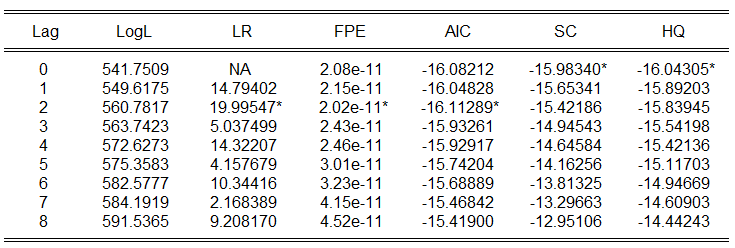
\includegraphics{laglength}}
\end{figure}
}


\subsection{Slide 5}
\frame{\frametitle{VAR and VECM Models - Slide 5}
\begin{itemize}
\item Undertaking diagnostics test on the residuals is a similar:
\end{itemize}
\begin{figure}
\caption{Diagnostics Tests}
    \scalebox{.3}{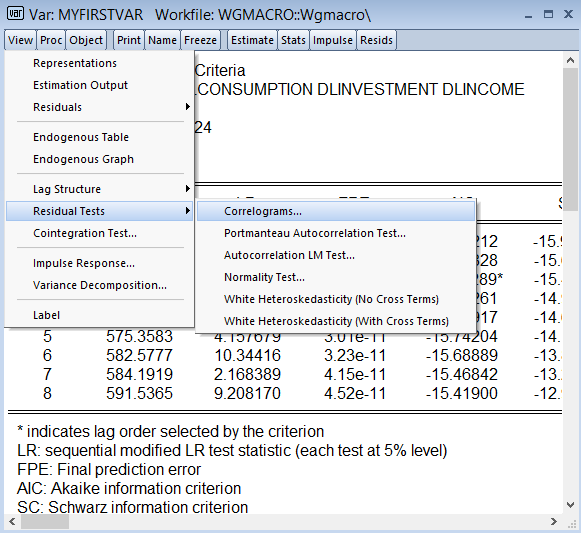
\includegraphics{diagnostics}}
\end{figure}
}

\subsection{Slide 6}
\frame{\frametitle{VAR and VECM Models - Slide 6}
\begin{itemize}
\item To undertake causality testing: `View` $\rightarrow$ `Lag Structure' $\rightarrow$ `Granger causality/block exogeneity':
\begin{equation*}
\textrm{H}_0:\beta_ 1 = \hdots = \beta_ i = 0
\end{equation*}
\begin{equation*}
\textrm{H}_1\textrm{: at least one}\neq
\end{equation*}
\begin{figure}
    \scalebox{.2}{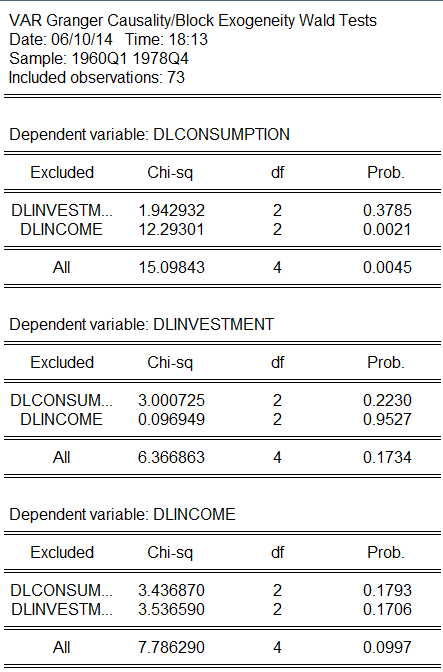
\includegraphics{granger}}
\end{figure}
\item \textbf{Quiz:} Can you see$\backslash$show how this is equivalent to Wald tests?
\end{itemize}
}

\subsection{Slide 7}
\frame{\frametitle{VAR and VECM Models - Slide 7}
\begin{itemize}
\item To undertake a Johansen test: `View $\rightarrow$ Cointegration Test' in the VAR or GROUP objects.
\begin{figure}
\caption{Johansen Test}
    \scalebox{.25}{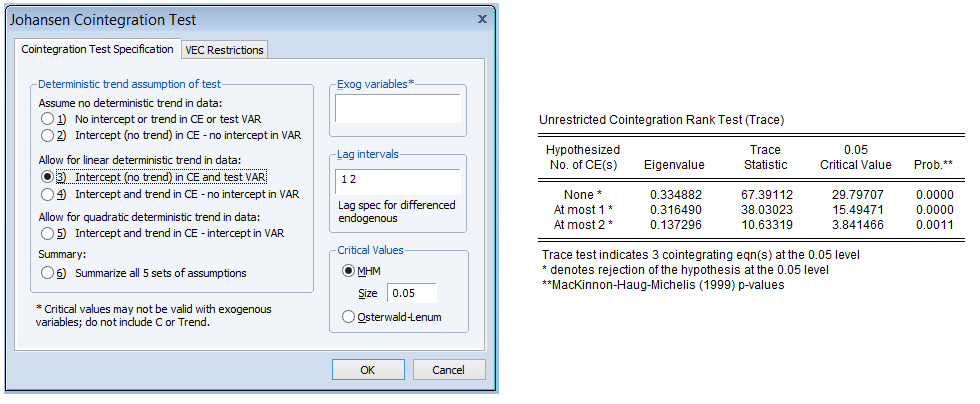
\includegraphics{cointtest}}
\end{figure}
\item To estimate a VECM requires an extremely similar command:\\[0.05in]
\small
\begin{center}
\color{blue}\texttt{var myfirstvecm.ec 1 2 dlconsumption dlinvestment dlincome}
\end{center}
\normalsize
\end{itemize}
}


\subsection{Slide 8}
\frame{\frametitle{VAR and VECM Models - Slide 8}
\begin{itemize}
\item From the VAR object: click - `Proc' $\rightarrow$ `Estimate'.\\[0.1in]
\item EViews has 5 different deterministic trend specifications.\\[0.1in]
\item To restrict the VECM is slightly more complicated.\\[0.1in]
\item Lets try an example with our `myfirstvecm' object to exclude income:\\[0.05in]
\begin{center}
\color{blue}
\texttt{
b(1,3)=0 , a(3,1)=0}
\color{black}
\begin{figure}
\caption{Restrictions}
\vspace{-0.05in}
    \scalebox{.2}{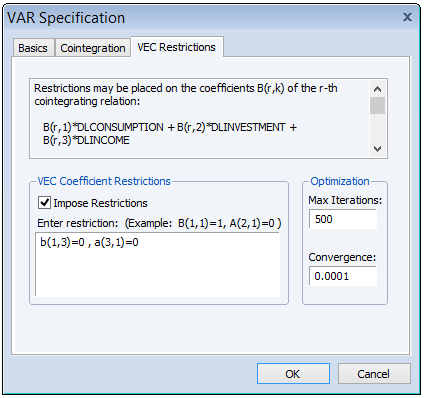
\includegraphics{restrict}}
\end{figure}
\end{center}
\end{itemize}
}


\subsection{Slide 9}
\frame{\frametitle{VAR and VECM Models - Slide 9}

There are two ways to forecast from VAR objects.
\begin{enumerate}
\item[1.] Directly through the VAR object (EViews 9.0 or later)
\item[2.]  Through the forecast add-in:\\[0.1in]
\end{enumerate}
\begin{itemize}
{\setlength\itemindent{15pt} \item Click on add-ins and download `fcast'}\\[0.05in]
{\setlength\itemindent{15pt} \item To forecast, return to the VAR object}\\[0.05in]
{\setlength\itemindent{15pt} \item Compare forecasts from the in-built option vs. add-in.}\\[0.05in]
{\setlength\itemindent{35pt} \item Do they match?}\\[0.05in]
{\setlength\itemindent{15pt} \item Try this with our `myfirstvar' and `myfirstvecm'.} \\[0.05in]
{\setlength\itemindent{35pt} \item Which is a better forecasting model?}\\[0.05in]
\end{itemize}
}

%\section{Eight}
%\subsection{Slide 1}
%\frame{\frametitle{Volatility Models - Slide 1}
%\begin{itemize}
%\item \textbf{A}uto\textbf{R}egressive \textbf{C}onditional \textbf{H}eteroskedasticity (ARCH) models are used when it is believed error terms will have a different variance.\\[0.1in]
%\item Assumes variance is a function of sizes of previous error terms.\\[0.1in]
%\begin{equation*}
%\varepsilon_t = \sigma_t z_t
%\end{equation*}
%\begin{equation*}
%\sigma_t^2 = \alpha_0 + \alpha_1 \varepsilon_{t-1}^2 + \hdots + \alpha_q \varepsilon_{t-q}^2
%\end{equation*}
%\item This model is typically estimated using least squares, with the lag length of the errors determined using a Lagrange test.\\[0.1in]
%\end{itemize}
%}
%
%\subsection{Slide 2}
%\frame{\frametitle{Volatility Models - Slide 2}
%\begin{itemize}
%\item Lets utilize data from the GETSTOCKS add-in for this section.\\[0.1in]
%\item Open a workfile from 1998/09/01 until 2014/06/01.\\[0.1in]
%\item Use GETSTOCKS to download BARX - Barclays stock data.\\[0.1in]
%\item Rename the close price to BARX: \\
%\begin{center}
%\color{blue} \texttt{rename barx\_close barx} \color{black}\\[0.1in]
%\end{center}
%\end{itemize}
%}
%\subsection{Slide 3}
%\frame{\frametitle{Volatility Models - Slide 3}
%\begin{itemize}
%\item The simplest way to estimate an ARCH is through the menus.\\[0.1in]
%\begin{figure}
%\caption{ARCH Models}
%\vspace{-0.05in}
%    \scalebox{.25}{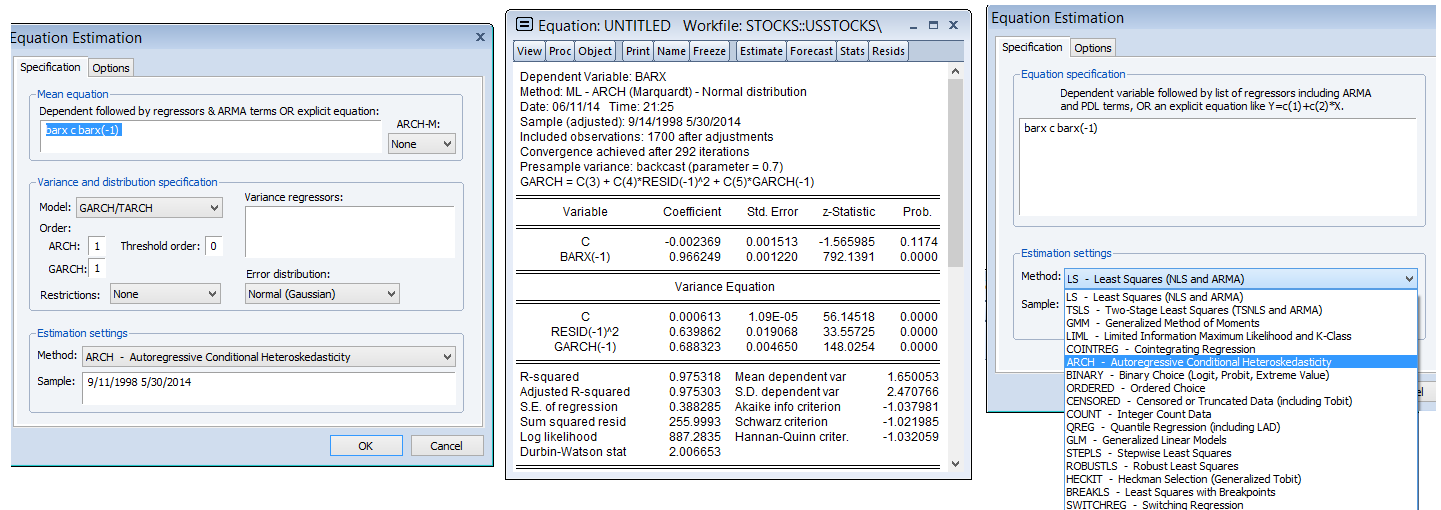
\includegraphics{arch}}
%\end{figure}
%\end{itemize}
%}
%
%\subsection{Slide 4}
%\frame{\frametitle{Volatility Models - Slide 4}
%\begin{itemize}
%\item From the previous slide, we can see how to specify the p, q paremters of a GARCH(p,q) model.\\[0.1in]
%\item If we want to include more lags (e.g. `x' lags) in mean equation:
%\begin{center}
%\color{blue}
%\texttt{ barx c barx(-1 to -x)}
%\end{center}
%\color{black}
%\item We can also input a variance/standard deviation into the mean equation (ARCH-M).\\[0.1in]
%\item EViews also offers options to estimate variants (e.g. EGARCH/TGARCH).\\[0.1in]
%\item We can also change the assumptions on the error distribution.\\[0.1in]
%\end{itemize}
%}
%
%\subsection{Slide 5}
%\frame{\frametitle{Volatility Models - Slide 5}
%\begin{itemize}
%\item We can also use the command line/programming envirnment:
%\color{blue}
%\begin{center}
%\texttt{equation eq1.arch barx c\\
%eq1.makegarch cvar\\
%plot cvar$^{.5}$\\
%}
%\end{center}
%\begin{figure}
%\caption{ARCH Models}
%    \scalebox{.09}{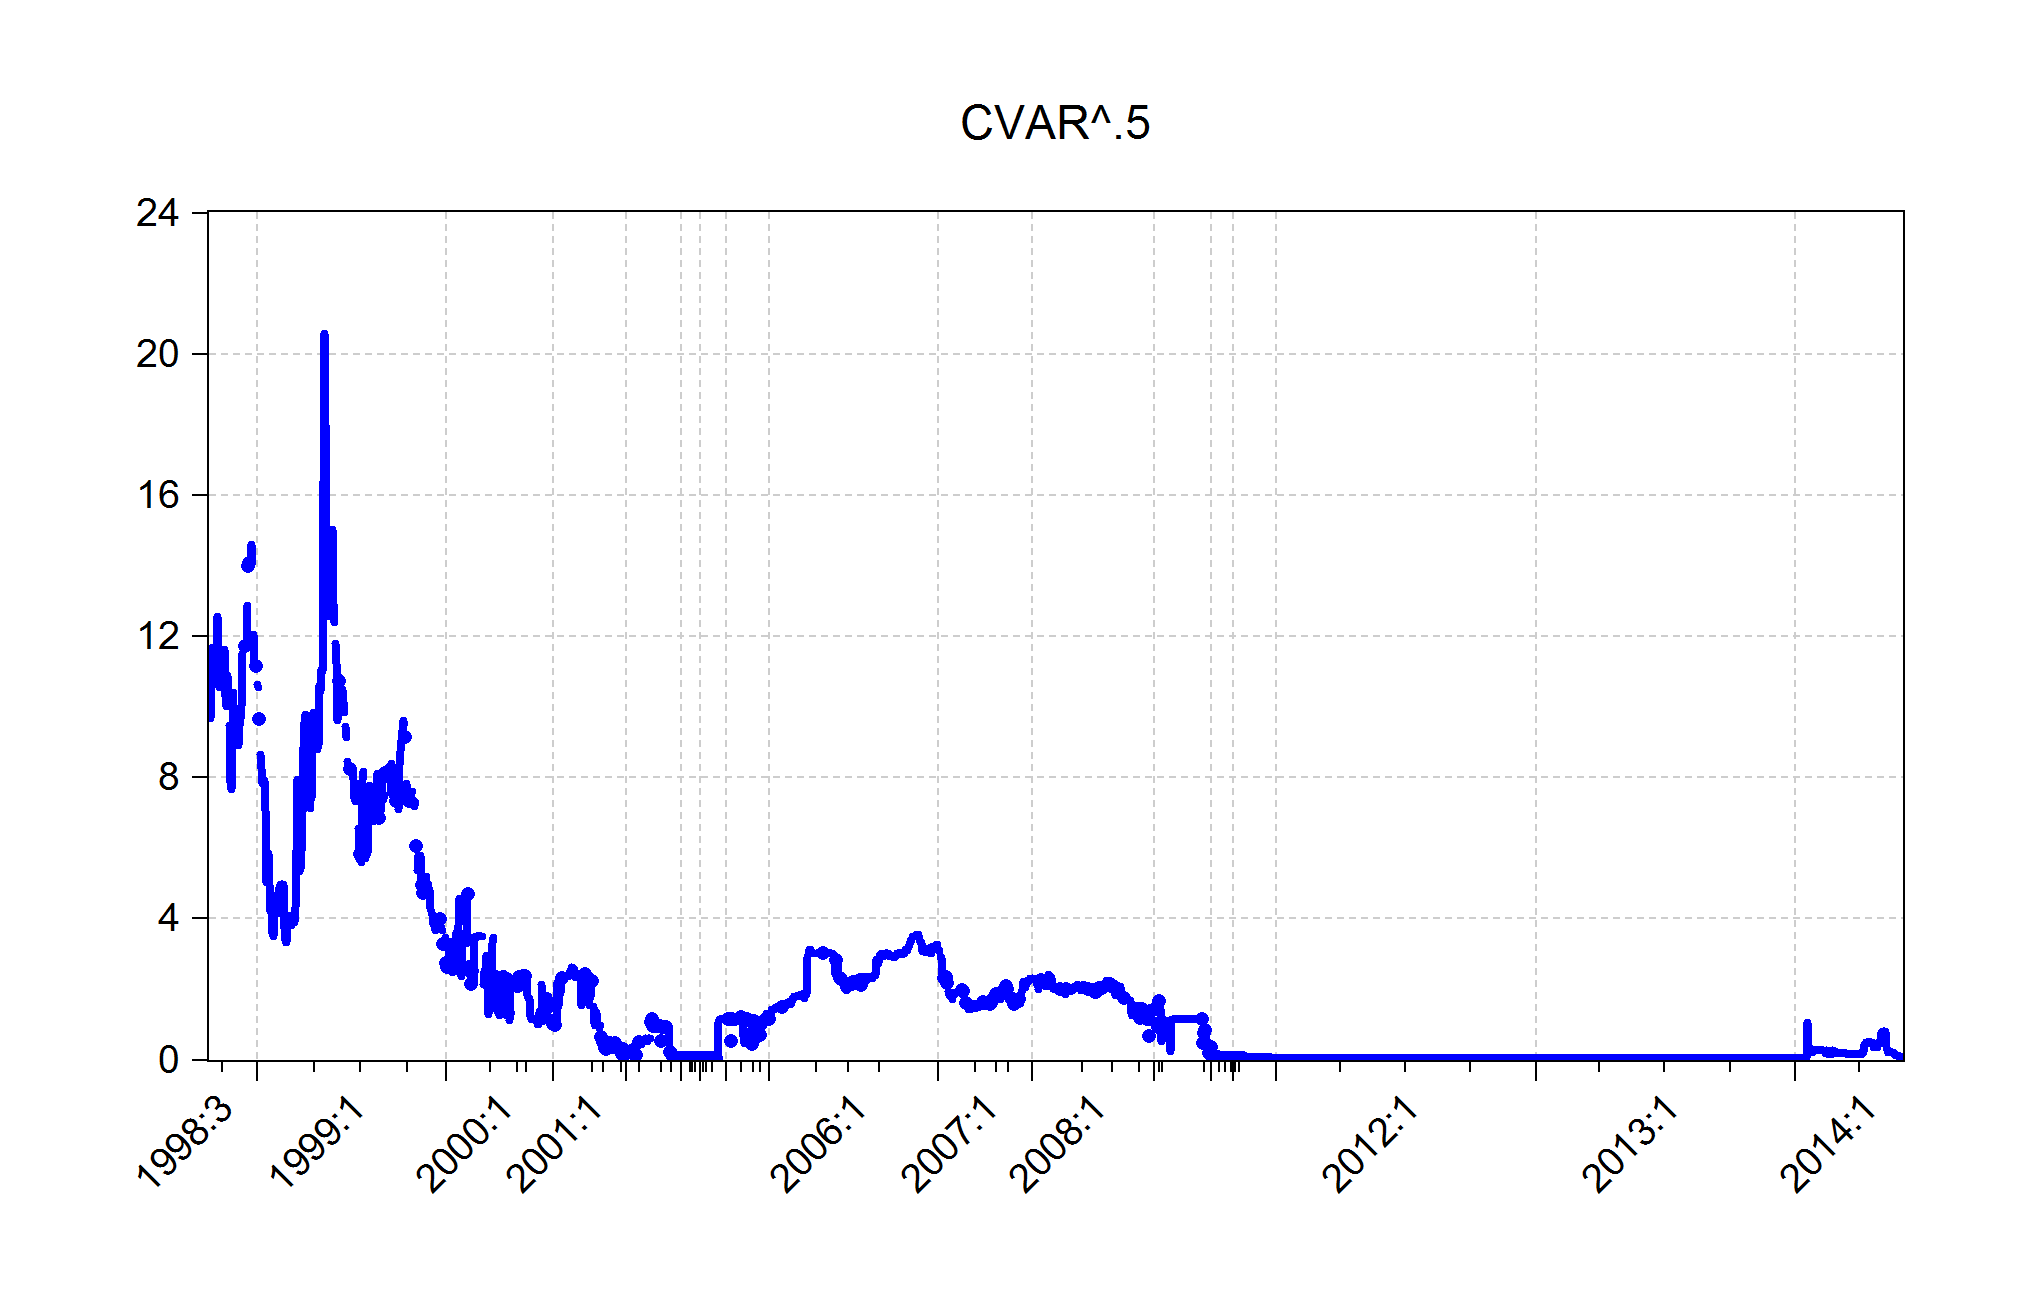
\includegraphics{barx}}
%\end{figure}
%\color{black}
%\end{itemize}
%}



\definecolor{mygreen}{RGB}{34,139,34}
\section{Programming}
\subsection{Slide 1}
\frame{\frametitle{An Introduction to Programming - Slide 1}
\begin{itemize}
\item The best way to learn any programming language is to see some basic examples doing various things and then work through them line by line.\\[0.1in]
\item Each of the following programs should work if you simply copy and paste them into a new program window and run them.\\ [0.1in]
\item Alternatively, you can save them as .prg files (in notepad/notepad++). Double clicking them should run them automatically.\\[0.1in]
\item  \color{mygreen}' \color{black}Indicates something commented out. \color{mygreen} Comments always appear in green. \color{black} These never effect how the program executes. Always include many comments in your own programs for any software!\\[0.1in]
\item Anything in \color{blue}blue \color{black} is part of a control statement (\color{blue}if\color{black}, \color{blue} for\color{black}, \color{blue}while\color{black}).
\end{itemize}	
}


\subsection{Slide 2}
\frame{\frametitle{An Introduction to Programming - Slide 2}
\small{Our first program creates a (normally distributed) Y series and 10 X series and regresses each X on Y with a constant:}\\ [.25in]
%\begin{shaded}
\hspace{30mm}\textbf{Generating data and FOR loops}\\ [.1in]
\scriptsize
\color{black}
\texttt{
\hspace{28.5mm}create a workfile\\
\hspace{30mm}wfcreate m 1900 2010 \color{mygreen}`create y and 10 X series\color{black}\\
\hspace{30mm}series y=nrnd\\
\hspace{30mm}\color{blue}for\color{black} !i=1 to 10\\
\hspace{35mm}series x\{!i\}=nrnd\\
\hspace{30mm}\color{blue}next \color{mygreen}`pairwise regressions between Y and each X\color{blue}\\
\hspace{30mm}\color{blue}for\color{black} !i=1 to 10\\
\hspace{35mm}equation eq\{!i\}.ls y c x\{!i\}\\
\hspace{30mm}\color{blue}next\\ [.3in]
}
\color{black}
\small{\textbf{Quiz:} Why does the for loop run from !i = 1 to 10?}
}

\subsection{Slide 3}
\frame{\frametitle{An Introduction to Programming - Slide 3}
\small{Using FOR loops to generate recursive (with an natural extension to rolling) estimations:}\\ [.25in]
\hspace{30mm}\textbf{A Simple Recursive Estimation}\\ [.1in]
\scriptsize
\color{black}
\texttt{
\hspace{28.5mm}create undated 1000\\
\hspace{30mm}series y=nrnd\\
\hspace{30mm}series x=nrnd\\
\hspace{30mm}\color{blue}for\color{black} !j=1 to 100\\
\hspace{35mm}smpl @first 900+!j\\
\hspace{35mm}equation eq\_\{!j\}.ls y x c\\
\hspace{30mm}\color{blue}next\color{black}\\
\hspace{30mm}smpl @all `\color{mygreen} Why do we do this?\\ [.3in]
}
\color{black}
\small{\textbf{Quiz:} What do the @first and 900+!j represent?}
}

\subsection{Slide 4}
\frame{\frametitle{An Introduction to Programming - Slide 4}
\small{Now we'll create a program which generates 10 X's and generates each on each other using \emph{double} for loops:}\\ [.25in]
\hspace{30mm}\textbf{Double FOR loops}\\[0.1in]
\scriptsize
\color{black}
\texttt{
\hspace{28.5mm}wfcreate m 1900 2010\\
\hspace{30mm}\color{blue}for\color{black} !i=1 to 10\\
\hspace{35mm}series x\{!i\}=nrnd\\
\hspace{30mm}\color{blue}next\\
\hspace{30mm}\color{blue}for\color{black} !i=1 to 9\\
\hspace{35mm}\color{blue}for\color{black} !j=!i+1 to 10\\
\hspace{40mm}equation eq\{!i\}\_\{!j\}.ls x\{!i\} c x\{!j\}\\
\hspace{35mm}\color{blue}next\color{black}\\
\hspace{30mm}\color{blue}next\color{black}\\ [.3in]
}
\color{black}
\small{\textbf{Quiz:} Why does the !j for loop include !i?}
}


\subsection{Slide 5}
\frame{\frametitle{An Introduction to Programming - Slide 5}
Now create a matrix to store the coefficients:\\ [.25in]
\hspace{30mm}\textbf{Storing Coefficients}\\[0.1in]
\scriptsize
\color{black}
\texttt{
\hspace{28.5mm}wfcreate m 1900 2010\\
\hspace{30mm}series y=nrnd\\
\hspace{30mm}\color{blue}for\color{black} !i=1 to 10\\
\hspace{35mm}series x\{!i\}=nrnd\\
\hspace{30mm}\color{blue}next\color{black}\\
\hspace{30mm}matrix(2,10) coefs\\
\hspace{30mm}equation eq\\
\hspace{30mm}\color{blue}for\color{black} !i=1 to 10\\
\hspace{35mm}eq.ls y c x\{!i\}\\
\hspace{35mm}colplace(coefs, eq.@coefs, !i)\\
\hspace{30mm}\color{blue}next\color{black}\\ [.3in]
}
\color{black}
\small{\textbf{Quiz:} Why do we need a matrix with dimension 2 by 10?}
}

\subsection{Slide 6}
\frame{\frametitle{An Introduction to Programming - Slide 6}
\small{Creating user friendly user interfaces:}\\ [.25in]
\hspace{10mm}\textbf{User Interfaces}\\[0.1in]
\scriptsize
\color{black}
\texttt{
\hspace{8.5mm}create undated 1000\\
\hspace{10mm}series y=nrnd\\
\hspace{10mm}series x=nrnd\\
\hspace{10mm}series w=nrnd\\
\hspace{10mm}\%dep = ""   \color{mygreen}`store name of dependent variable\color{black}\\
\hspace{10mm}\%regs = "c "  \color{mygreen}`store list of regressors.  Default is "c".\color{black}\\
\hspace{10mm}!result  = 0   \color{mygreen}` variable that will track the result of dialogs.\color{black}\\
\hspace{10mm}!result = @uiedit(\%dep,"Enter dependent variable")  \color{mygreen}` Ask for dependent.\color{black}\\
\hspace{10mm}!result = @uiedit(\%regs,"Enter the list of regressors") \color{mygreen}` Ask for regressors.\color{black}\\
\hspace{10mm}equation eq1.ls {\%dep} {\%regs}   \color{mygreen}`estimate equation.\color{black}\\ [.3in]
}
\color{black}
\small{\textbf{Quiz:} Can you create an option to exit the routine through a UI?}
}


\section{Homework}
\subsection{Optional Homework}
\frame{\frametitle{Optional Homework Assignment}
\begin{enumerate}
\small
\item[1.] Download or import a foreign exchange rate (or alternatively, a portfolio of your creation) measured on a daily (or higher) frequency.\\
\item[2.] Write a program which estimates your portfolio/series as a GARCH model using a rolling scheme (see helpfiles for exact GARCH commands/options).\\
\item[3.] Choose a suitable window length (the sample which you use for estimating the coefficeints)/roll size. Consider advantages/disadvantages of various sizes.\\
\item[4.] Use your program to forecast the variance from each rolled estimation. Note the three fields available in ARCH type forecasts (s.e., volatility and mean), as detailed in the helpfiles).\\
\item[5.] (Time permitting) Calculate the value at risk from these forecasts and therefore calculate the failure rate of the model - that is - how many times do losses exceed the maximum losses predicted by VaR.\\[0.05in]
\item[6.] If you get stuck, try this helpful forum post by EViews staff:
\begin{center}
\color{blue}\url{http://forums.eviews.com/viewtopic.php?f=15&t=878}
\end{center}
\end{enumerate}
}
\end{document}	